\documentclass[12pt]{article}
\usepackage[a4paper, top=1.1in, bottom=1.1in, left=1.25in, right=1.25in]{geometry}
\usepackage{lmodern}
\usepackage[T1]{fontenc}
\usepackage{amsmath}
\usepackage{booktabs}
\usepackage{listings}
\usepackage{xcolor}
\usepackage{graphicx}
\usepackage{float}
\usepackage[hidelinks]{hyperref}
\linespread{1.1}
\setlength{\parskip}{0.5em}

\definecolor{codebg}{RGB}{248,248,248}
\definecolor{codeframe}{RGB}{200,200,200}

\lstdefinestyle{plain}{
  backgroundcolor=\color{codebg},
  frame=single,
  rulecolor=\color{codeframe},
  basicstyle=\small\ttfamily,
  showstringspaces=false,
  breaklines=true,
  xleftmargin=1em,
  framexleftmargin=0.5em,
}

\setlength{\parindent}{0pt}

\renewcommand{\thesection}{\arabic{section}.}
\renewcommand{\thesubsection}{\thesection\arabic{subsection}.}

\title{End-to-End Performance Engineering\\of Google Online Boutique}
\author{Muhammad Sohail (7178621) \\ Syed Umair Anwar (7172248)}
\date{\today}

\begin{document}

\maketitle
\begin{center}
\small
\textbf{Course:} SOFTWARE PERFORMANCE ENGINEERING 2025--2026 \\[2pt]
\textbf{Case Study:} End-to-End Case Study (Project 7) \\[2pt]
\textbf{Benchmark:} Google Online Boutique (microservices-demo) \\[2pt]
\textbf{Fork:} \url{https://github.com/msohailse/microservices-demo-spe}
\end{center}
\thispagestyle{empty}
\newpage

\tableofcontents
\newpage

% ──────────────────────────────────────────
\section{Project Overview}

This report documents a comprehensive performance engineering study of the Google Online Boutique, a cloud-native microservice benchmark application. The study covers the full pipeline: deployment, workload measurement, analytical modelling via Queueing Networks (QN/LQN), and performance optimization.

% ──────────────────────────────────────────
\section{System Architecture}

Google Online Boutique consists of 11 microservices written in multiple languages, deployed on Kubernetes. The services communicate via gRPC.

\begin{figure}[h]
  \centering
  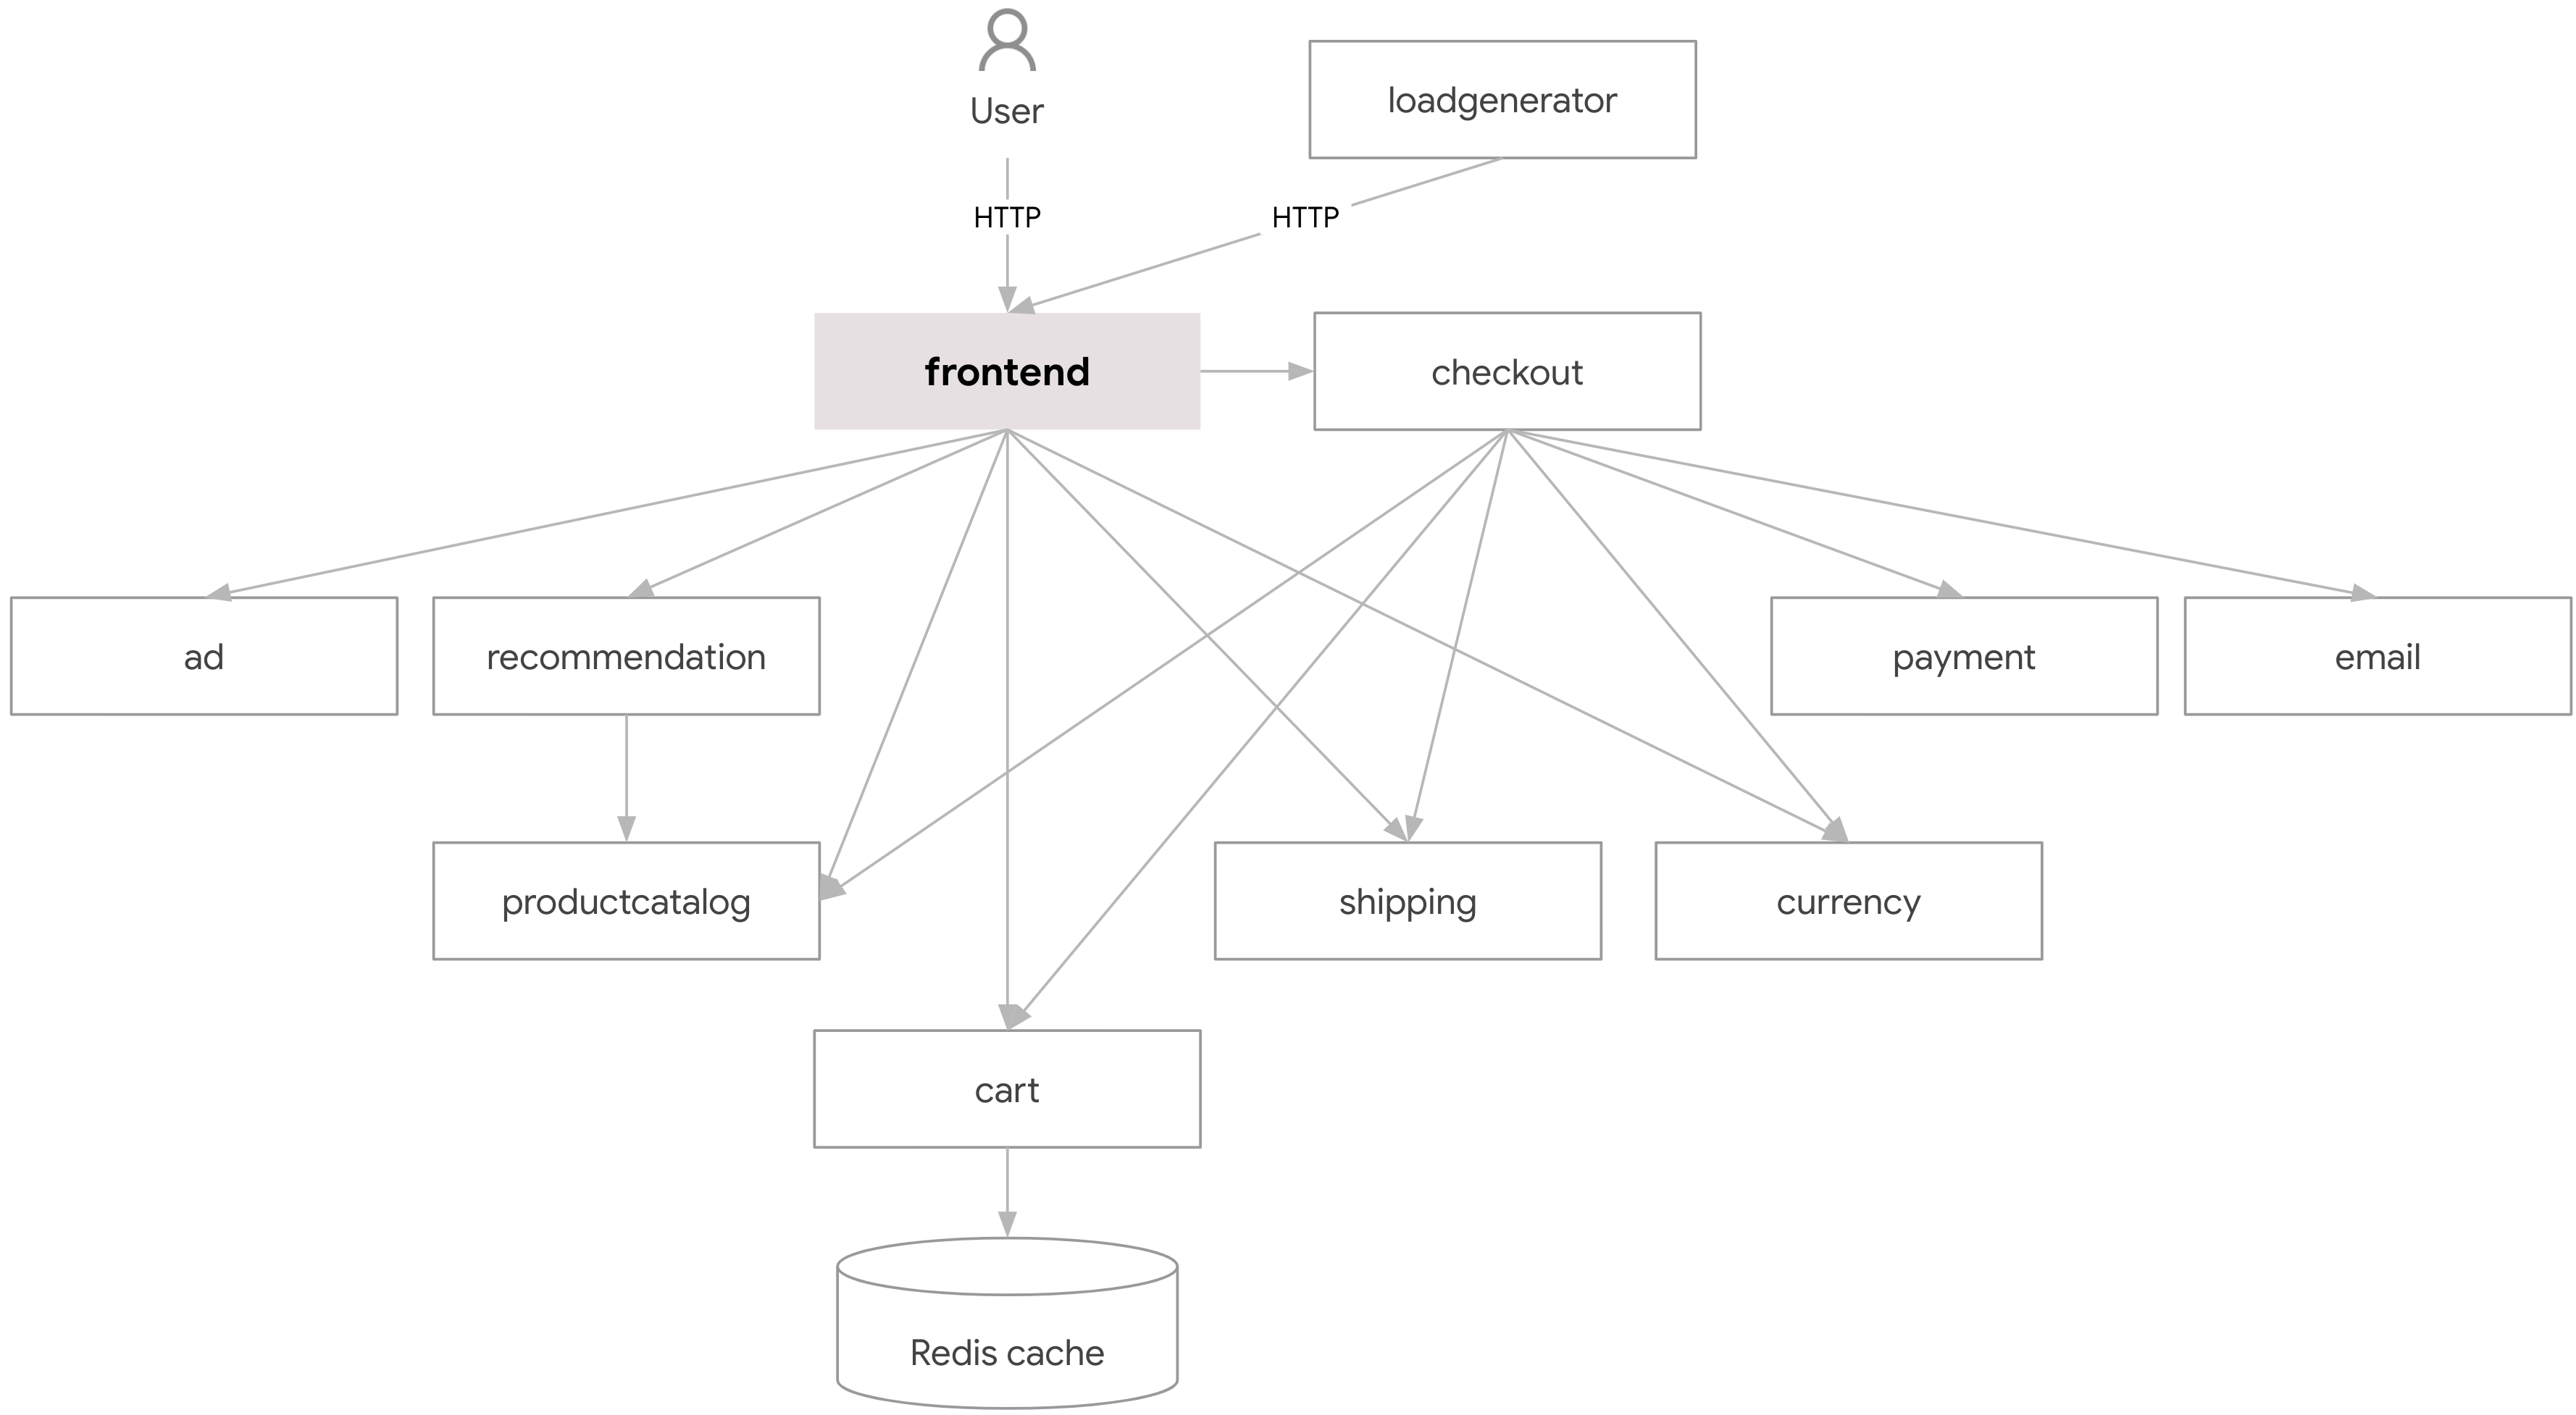
\includegraphics[width=0.9\textwidth]{screenshots/architecture.png}
  \caption{Google Online Boutique architecture (source: GoogleCloudPlatform/microservices-demo)}
\end{figure}

% ──────────────────────────────────────────
\section{Setup and Deployment}

\subsection{Environment}

\begin{itemize}
  \item Minikube with Docker driver, 6 CPUs, 9 GB memory
  \item Helm for monitoring stack deployment
\end{itemize}

\subsection{Deployment}

\begin{lstlisting}[style=plain]
minikube start --driver=docker --cpus=6 --memory=9g
kubectl apply -f release/kubernetes-manifests.yaml
\end{lstlisting}

\begin{figure}[h]
  \centering
  
\includegraphics[width=0.95\textwidth]{screenshots/deploy-complete.png}
  \caption{\texttt{./scripts/deploy.sh} completion output: all services deployed and port-forward commands printed for Grafana, Prometheus, and Jaeger.}
  \label{fig:deploy-complete}
\end{figure}

\subsection{Fork Fix: Resource Limits for Minikube Stability}

The study uses a fork of the benchmark that also includes all measurement and deployment scripts (\url{https://github.com/msohailse/microservices-demo-spe}). The upstream manifests set CPU limits (\texttt{300m} for \texttt{cartservice}, \texttt{150m} for \texttt{currencyservice}) tuned for GKE node pools, which caused \texttt{CrashLoopBackOff} on Minikube: both services are CPU-intensive at startup (\texttt{cartservice} runs .NET JIT warmup; \texttt{currencyservice} has a single-threaded Node.js event loop), and the original caps throttled them before they could respond to their gRPC liveness probes. The fork increases these limits to \texttt{600m} and \texttt{300m} respectively and raises memory to \texttt{256Mi}, giving each container the burst headroom to pass health checks reliably. All performance measurements in this report are taken after this fix is in place. While this infrastructure fix restores system stability, it increases the baseline computational cost of the cluster by allocating an additional 300\,m CPU to \texttt{cartservice} and 150\,m CPU to \texttt{currencyservice}.

\begin{table}[H]
  \centering
  \begin{tabular}{lcc}
    \toprule
    Metric & Before fix (upstream limits) & After fix (increased limits) \\
    \midrule
    System status      & \texttt{CrashLoopBackOff}    & Stable \\
    System mean R (ms) & Failing                      & 38.6 \\
    System p95 (ms)    & Timeout / 500 Error          & 97.8 \\
    \bottomrule
  \end{tabular}
  \caption{Effect of increasing CPU limits on \texttt{cartservice} (300\,m $\to$ 600\,m) and \texttt{currencyservice} (150\,m $\to$ 300\,m). Before values reflect the upstream configuration where liveness probe failures caused \texttt{CrashLoopBackOff}; after values are empirical measurements from Prometheus at baseline load ($N{=}10$, RATE=1).}
  \label{tab:fix}
\end{table}

\subsection{Monitoring Stack}

Prometheus and Grafana deployed inside the cluster via Helm (kube-prometheus-stack). Prometheus auto-discovers all pods via Kubernetes service discovery. Grafana connects to Prometheus for dashboards. Port-forwarding tunnels browser access into the minikube network.

\begin{lstlisting}[style=plain]
./scripts/monitoring-setup.sh
\end{lstlisting}

Access Grafana via port-forward at \texttt{localhost:3000}, username \texttt{admin}. The chart generates a random admin password on each fresh install rather than a fixed default, retrievable via:

\begin{lstlisting}[style=plain]
kubectl --namespace monitoring get secrets monitoring-grafana \
  -o jsonpath="{.data.admin-password}" | base64 -d; echo
\end{lstlisting}

\subsection{Distributed Tracing (Jaeger + Istio)}

Per the assignment's Guidelines and Best Practices, tracing is required both for dependency-graph extraction and to capture routing probabilities and per-service demands used in the QN/LQN model. Rather than instrumenting each of the 11 services individually with OpenTelemetry SDK calls, tracing is obtained for free from the service mesh already used in this deployment: Istio injects an Envoy sidecar proxy into every pod, and each sidecar reports a trace span for every request it forwards, with no application code changes.

\textbf{Deployment order matters.} Istio's sidecar injection is decided once, at pod-creation time, based on a namespace label. The pipeline therefore enables Istio and applies the tracing configuration \emph{before} the application pods exist, so every one of the 11 services comes up already wrapped in a sidecar and already pointed at a tracing backend:

\begin{lstlisting}[style=plain]
./scripts/monitoring-setup.sh                       # (1) Istio + injection label + Prometheus/Grafana
kubectl apply -f monitoring-manifests/monitoring.yaml  # (2) Jaeger + Istio Telemetry resource
kubectl apply -f release/kubernetes-manifests.yaml     # (3) 11 microservices (sidecars auto-injected)
kubectl apply -f release/istio-manifests.yaml          # (4) Gateway/HTTPRoute exposing the frontend
\end{lstlisting}

\textbf{Components:}
\begin{itemize}
  \item \textbf{Jaeger} (\texttt{jaegertracing/all-in-one:1.60}), distributed tracing system deployed in the \texttt{monitoring} namespace.
  \item \textbf{jaeger-query}, a Kubernetes \texttt{Service} exposing port \texttt{16686}, giving Grafana and the browser a stable DNS name for Jaeger's UI/API instead of a pod IP.
  \item \textbf{Envoy sidecar (the ``Istio Proxy'')}, injected into every application pod. It does the physical work of capturing each request/response and forwarding the resulting span across the network to Jaeger; the application containers are unaware this is happening.
  \item \textbf{Zipkin format}, the common wire format both sides speak: Envoy has a built-in Zipkin trace exporter, and Jaeger's all-in-one image exposes a Zipkin-compatible receiver on port \texttt{9411}. An Istio \texttt{Telemetry} resource registers this Zipkin endpoint as the mesh's tracing provider (at 100\% sampling, since a benchmarking study needs every trace, not a 1\% production sample).
\end{itemize}

\textbf{Grafana/Prometheus wiring.} \texttt{monitoring-manifests/override\_values.yaml} is passed to the \texttt{kube-prometheus-stack} Helm release by \texttt{scripts/monitoring-setup.sh}. It adds Jaeger as a Grafana datasource and sets a 6-hour Prometheus retention window.

\begin{figure}[H]
  \centering
  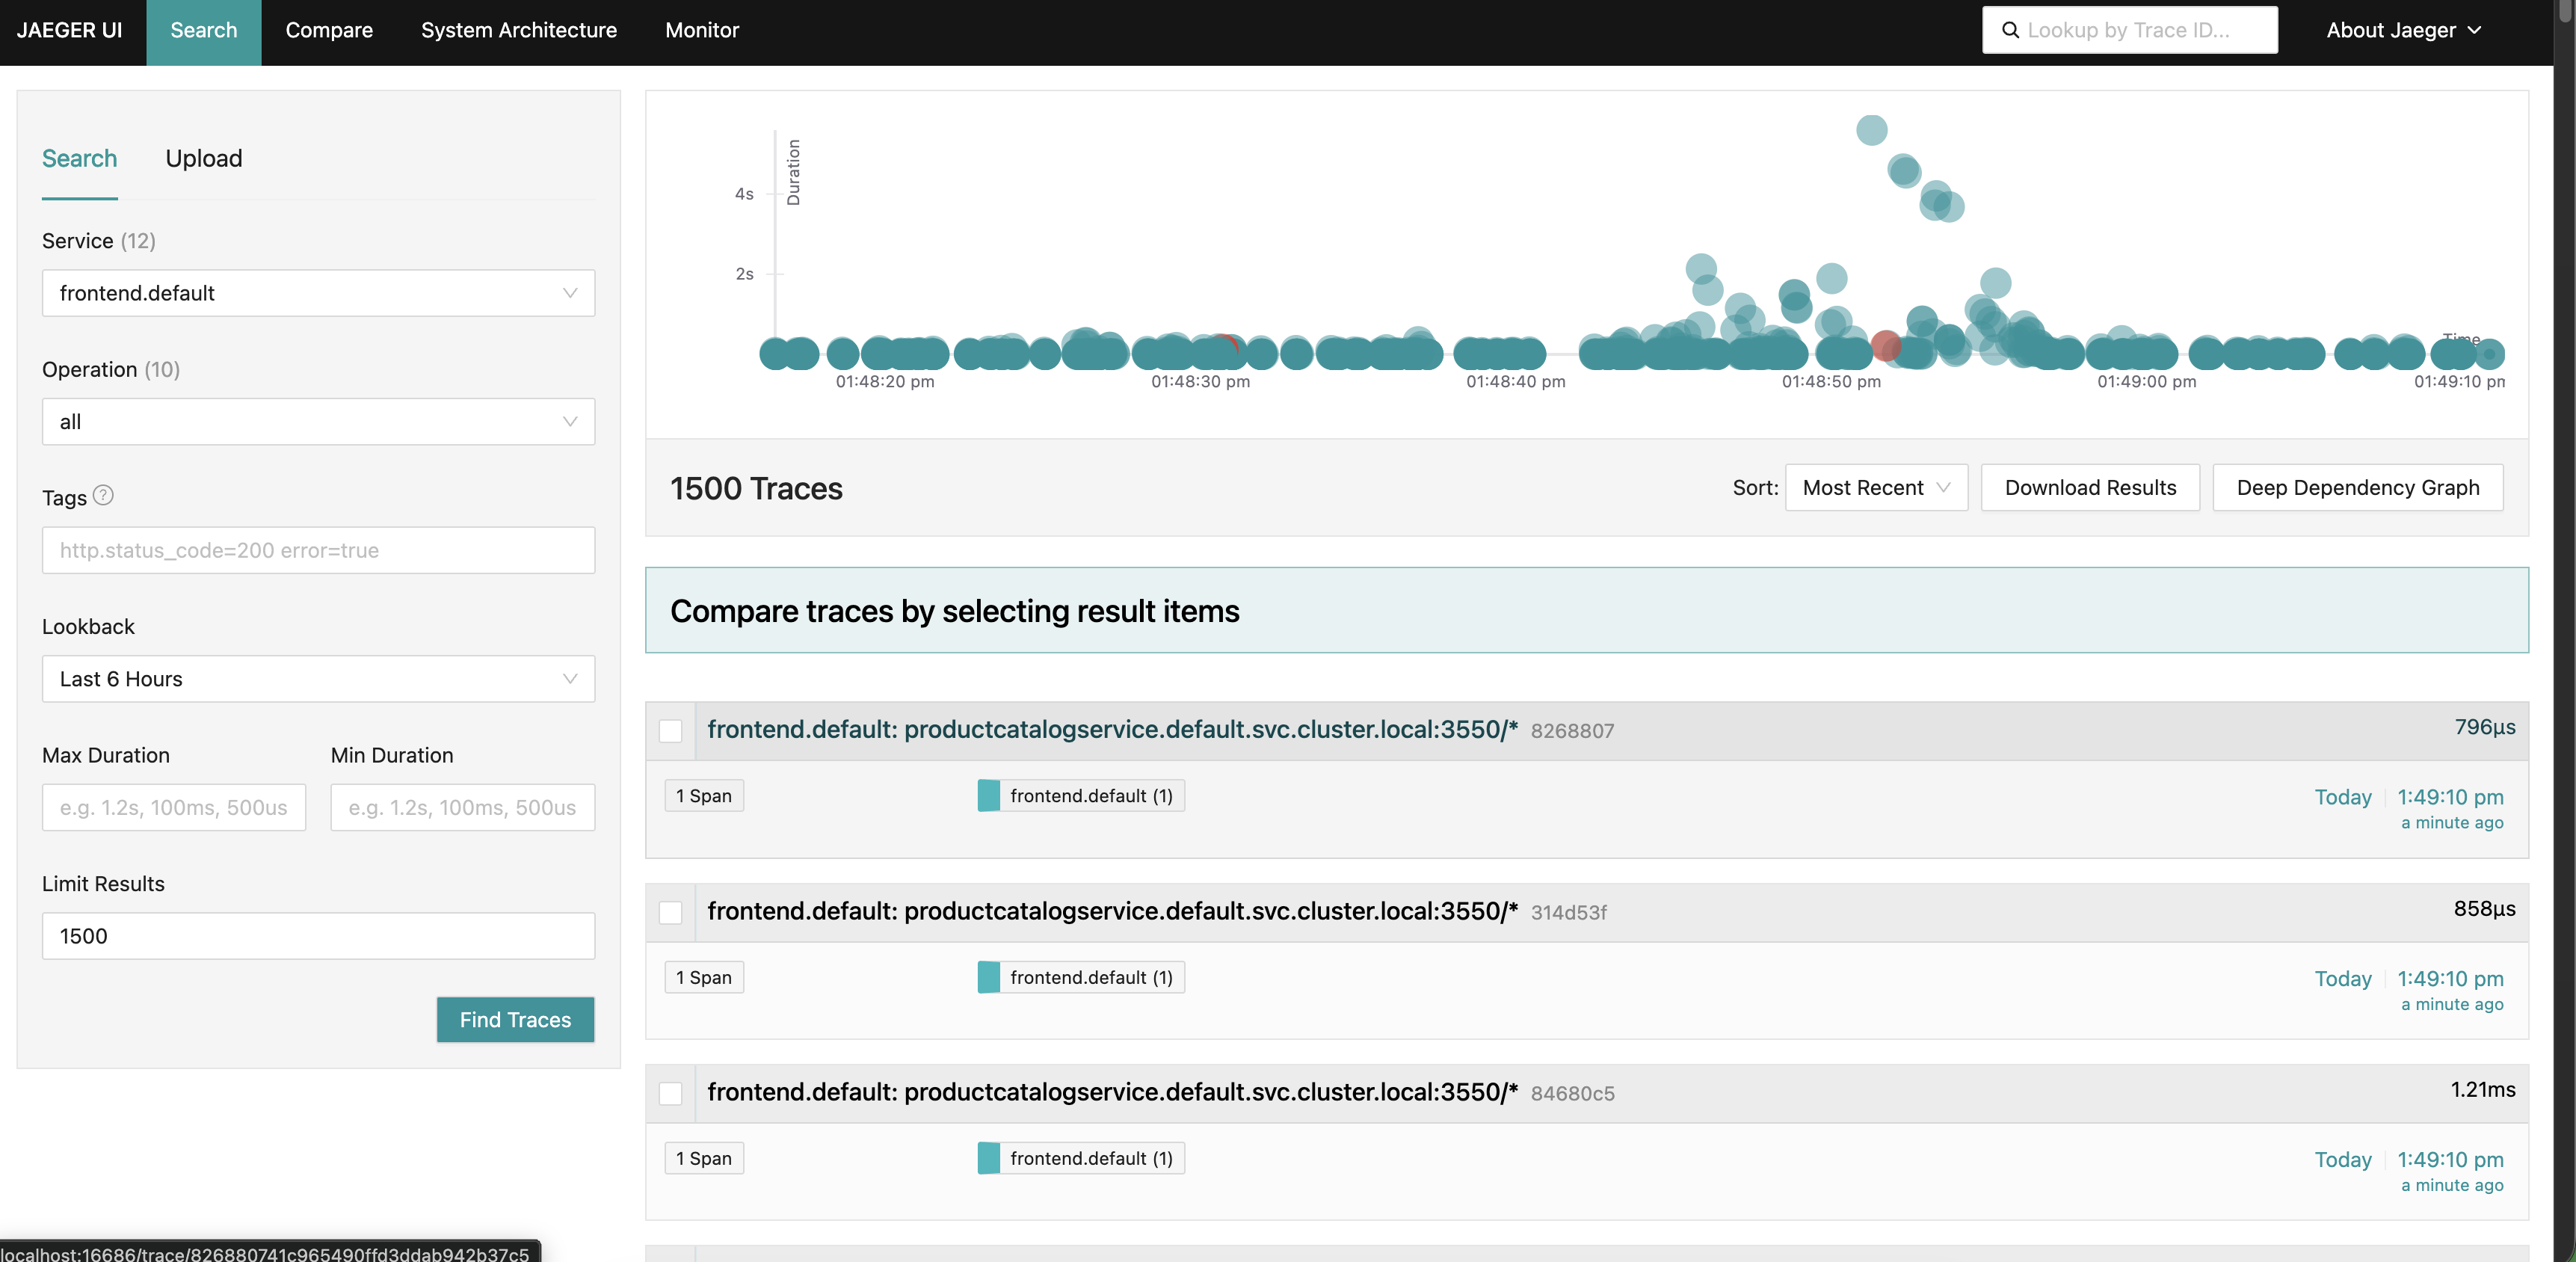
\includegraphics[width=0.95\textwidth]{screenshots/frontend-service-traces.png}
  \caption{Jaeger traces for \texttt{frontend}: 100\% sampling active under \texttt{loadgenerator} traffic.}
  \label{fig:frontend-traces}
\end{figure}

\begin{figure}[H]
  \centering
  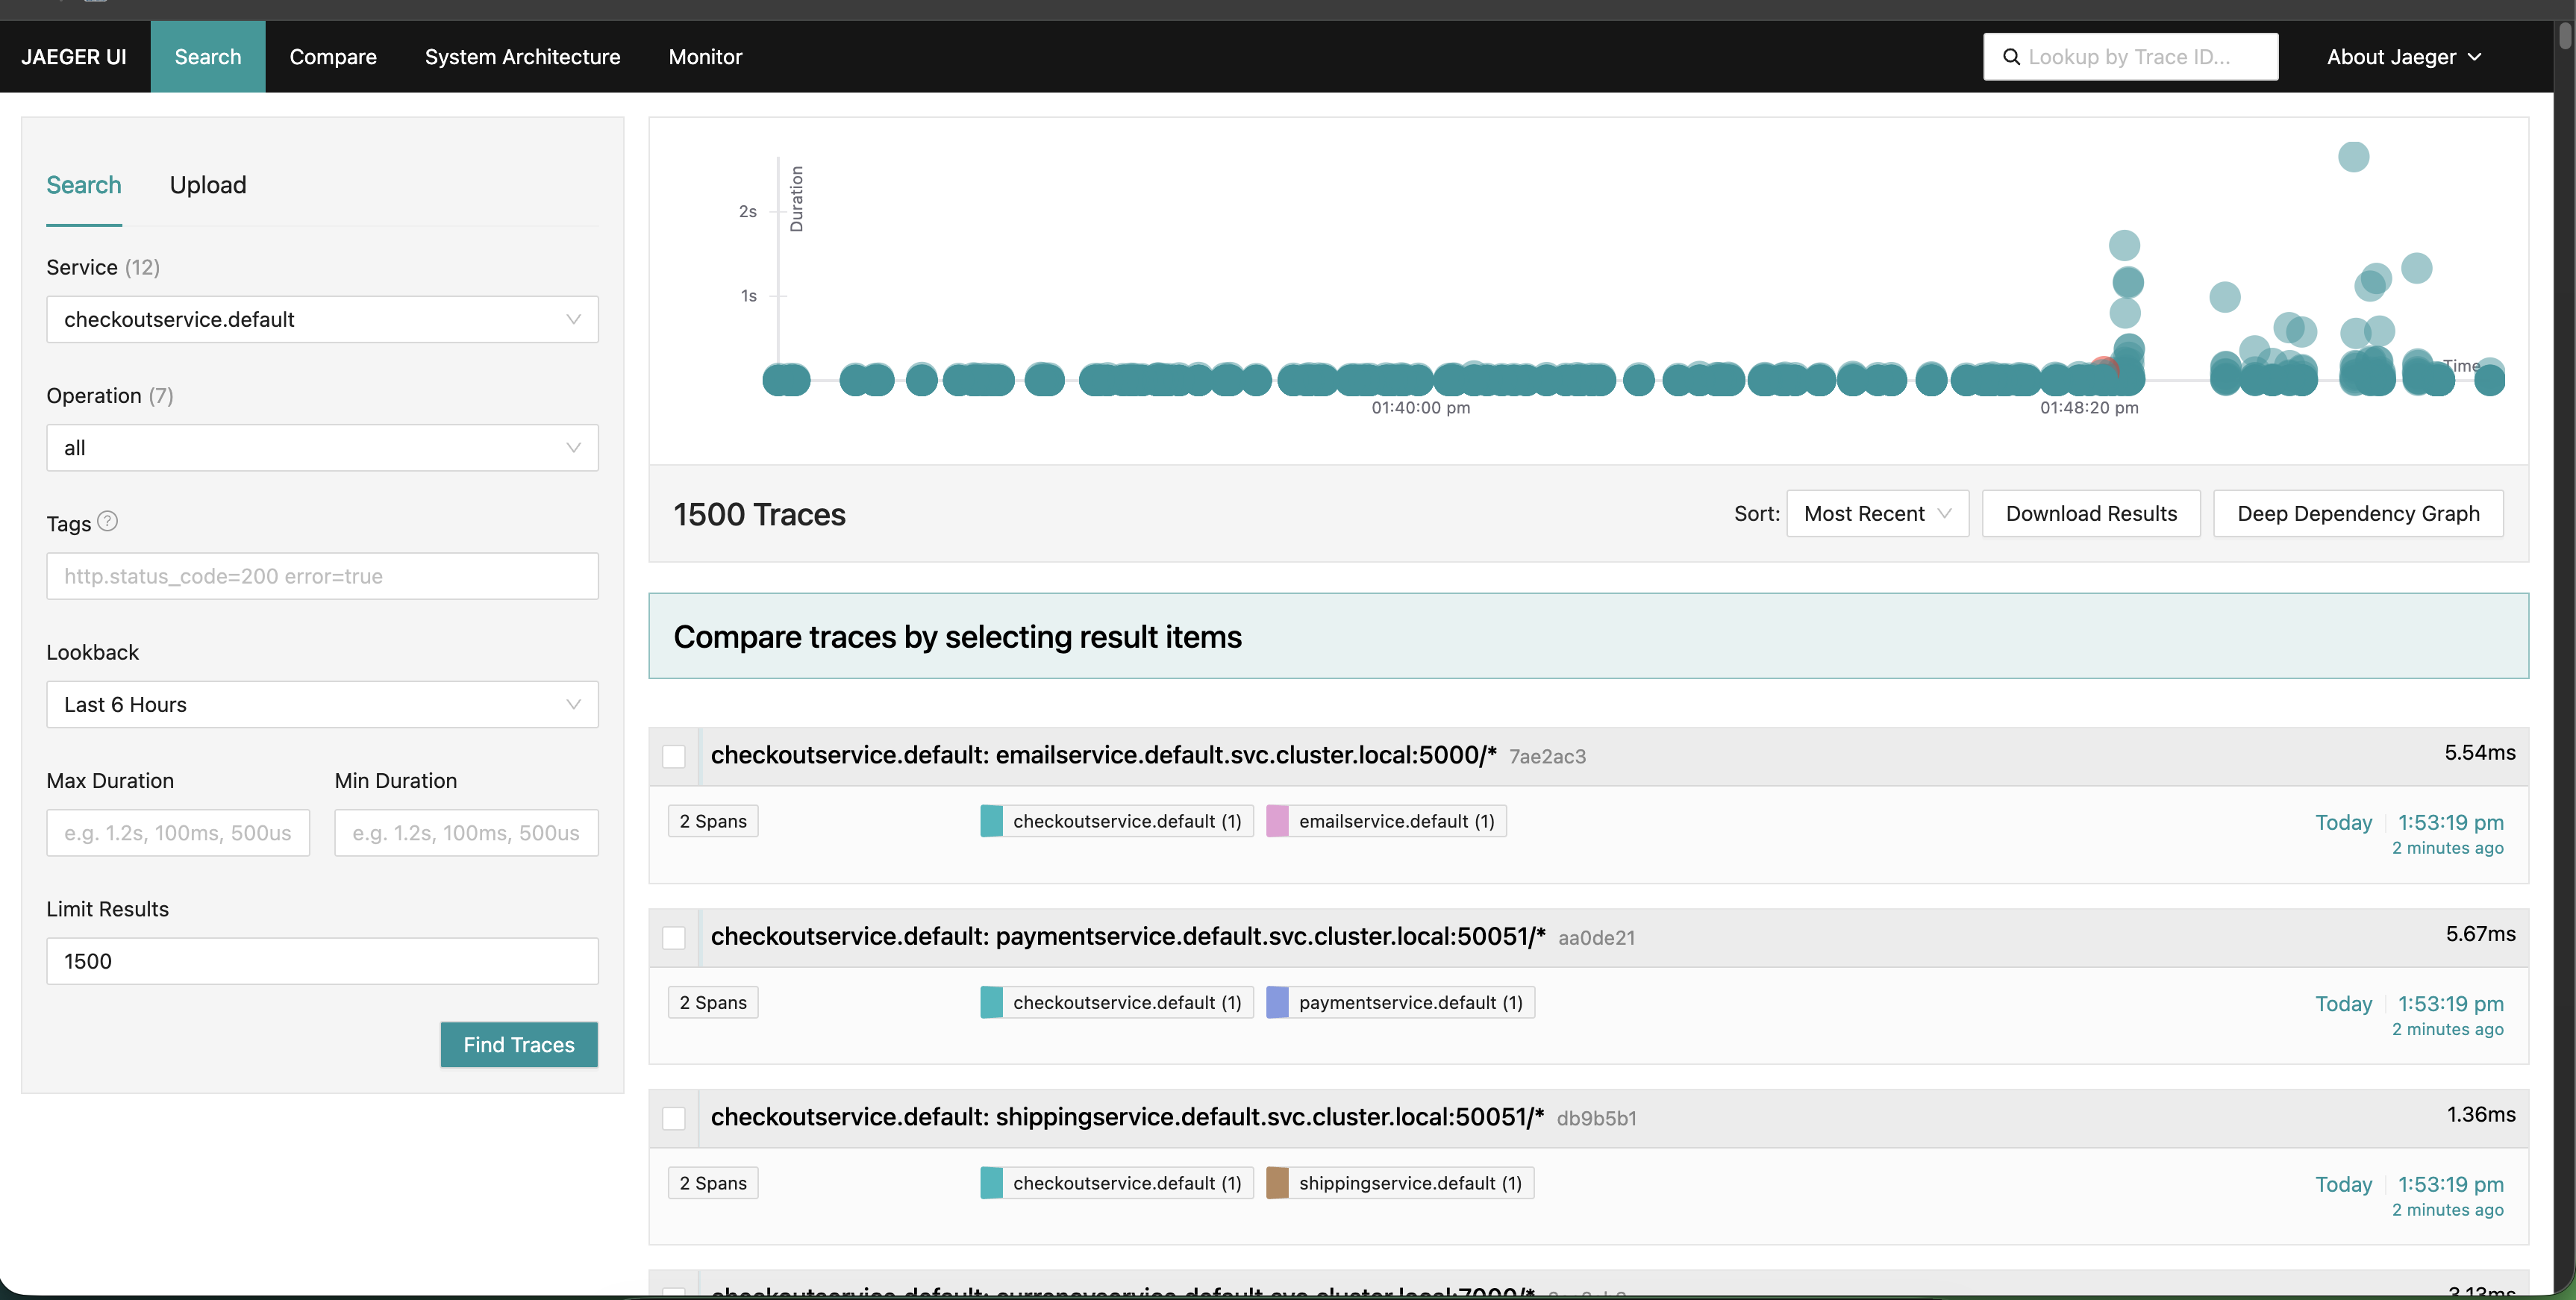
\includegraphics[width=0.95\textwidth]{screenshots/checkout-service-traces.png}
  \caption{Jaeger traces for \texttt{checkoutservice}: lower volume consistent with $V_{\text{checkoutservice}}=0.040$.}
  \label{fig:checkout-traces}
\end{figure}

% ──────────────────────────────────────────
\section{Workload Measurement}

\subsection{Load Generation}

Workload is generated by \texttt{loadgenerator}, a Locust-based deployment included in the upstream manifests. Four load levels were applied across this study:

\begin{itemize}
  \item Baseline: \texttt{USERS=10, RATE=1}
  \item Stress Test 1: \texttt{USERS=50, RATE=10}
  \item Stress Test 2: \texttt{USERS=100, RATE=10}
  \item Stress Test 3: \texttt{USERS=200, RATE=20}
\end{itemize}

\subsection{Metrics Collected}

All metrics originate from Envoy sidecars scraped via Prometheus — no application-level instrumentation was needed.

\textbf{Throughput / arrival rate ($\lambda$):}
\begin{lstlisting}[style=plain]
sum by (destination_workload) (rate(istio_requests_total[2m]))
\end{lstlisting}

\begin{table}[H]
  \centering
  \small
  \setlength{\tabcolsep}{5pt}
  \begin{tabular}{l|r|r|r|r|r}
    \toprule
    Service & $\lambda_i$ (req/s) & $S_{\text{meas}}$ (ms) & $S_{\text{net}}$ (ms) & $V_i$ & p95 (ms) \\
    \midrule
    productcatalogservice & 29.10 &  0.236 &  0.236 & 5.424 &   4.1 \\
    currencyservice       & 17.93 &  1.855 &  1.855 & 3.019 &   5.0 \\
    cartservice           &  5.87 &  1.876 &  1.876 & 0.968 &   4.9 \\
    frontend              &  5.77 & 32.837 & 17.126 & 1.000 &  97.8 \\
    recommendationservice &  4.00 &  8.985 &  8.749 & 0.716 &  24.3 \\
    adservice             &  3.37 &  1.305 &  1.305 & 0.567 &   4.9 \\
    shippingservice       &  1.97 &  0.659 &  0.659 & 0.292 &   4.6 \\
    paymentservice        &  0.33 &  3.462 &  3.462 & 0.037 &  17.5 \\
    checkoutservice       &  0.33 & 31.438 & 12.641 & 0.040 &  77.5 \\
    emailservice          &  0.33 &  3.462 &  3.462 & 0.036 &  17.5 \\
    \bottomrule
  \end{tabular}
  \caption{Baseline per-service measurements (USERS=10, $\lambda_{\text{root}}=5.22$ req/s): per-service arrival rate $\lambda_i$, measured residence time $S_{\text{meas}}$, net service time $S_{\text{net}}$ (downstream RPC wait subtracted via $S_{\text{net}}[s] = S_{\text{meas}}[s] - \sum_c f_{sc}\,S_{\text{net}}[c]$), visit ratio $V_i = \lambda_i / \lambda_{\text{root}}$, and 95th-percentile latency from Prometheus \texttt{histogram\_quantile}.}
  \label{tab:baseline-per-service}
\end{table}

\begin{figure}[H]
  \centering
  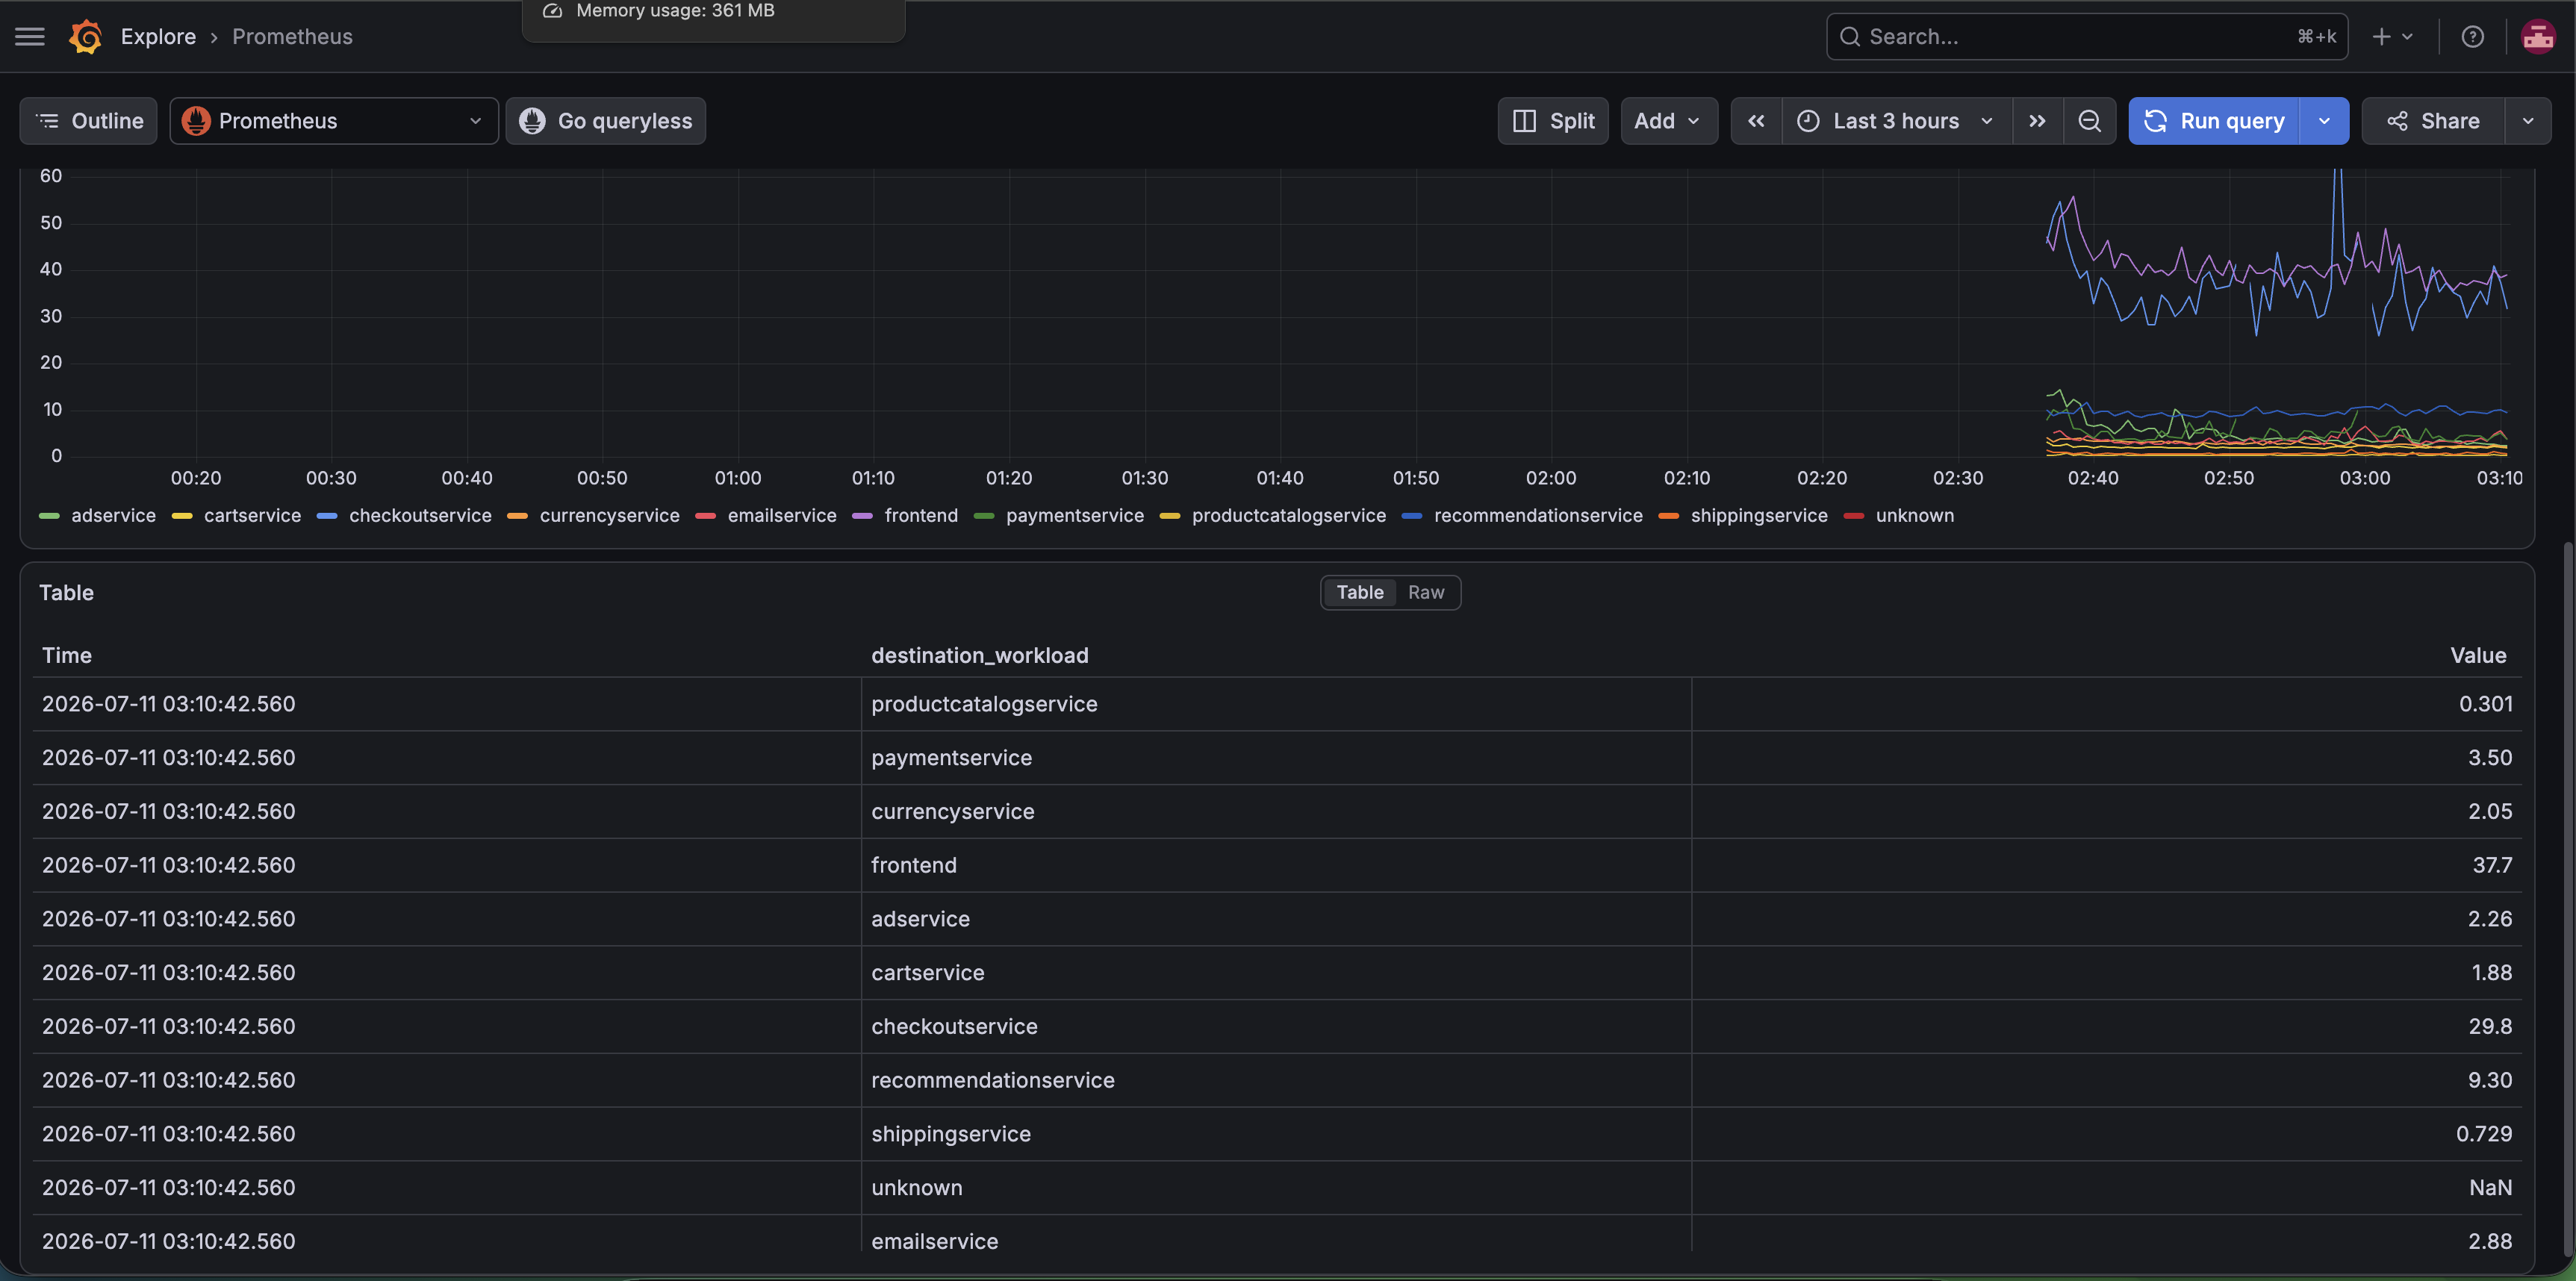
\includegraphics[width=0.95\textwidth]{screenshots/all_arrival_rate.png}
  \caption{All-services arrival rate (Prometheus API)}
  \label{fig:arrival-rates}
\end{figure}

\textbf{Mean service time:}
\begin{lstlisting}[style=plain]
sum by (destination_workload) (rate(istio_request_duration_milliseconds_sum[2m]))
  / sum by (destination_workload) (rate(istio_request_duration_milliseconds_count[2m]))
\end{lstlisting}

\begin{figure}[H]
  \centering
  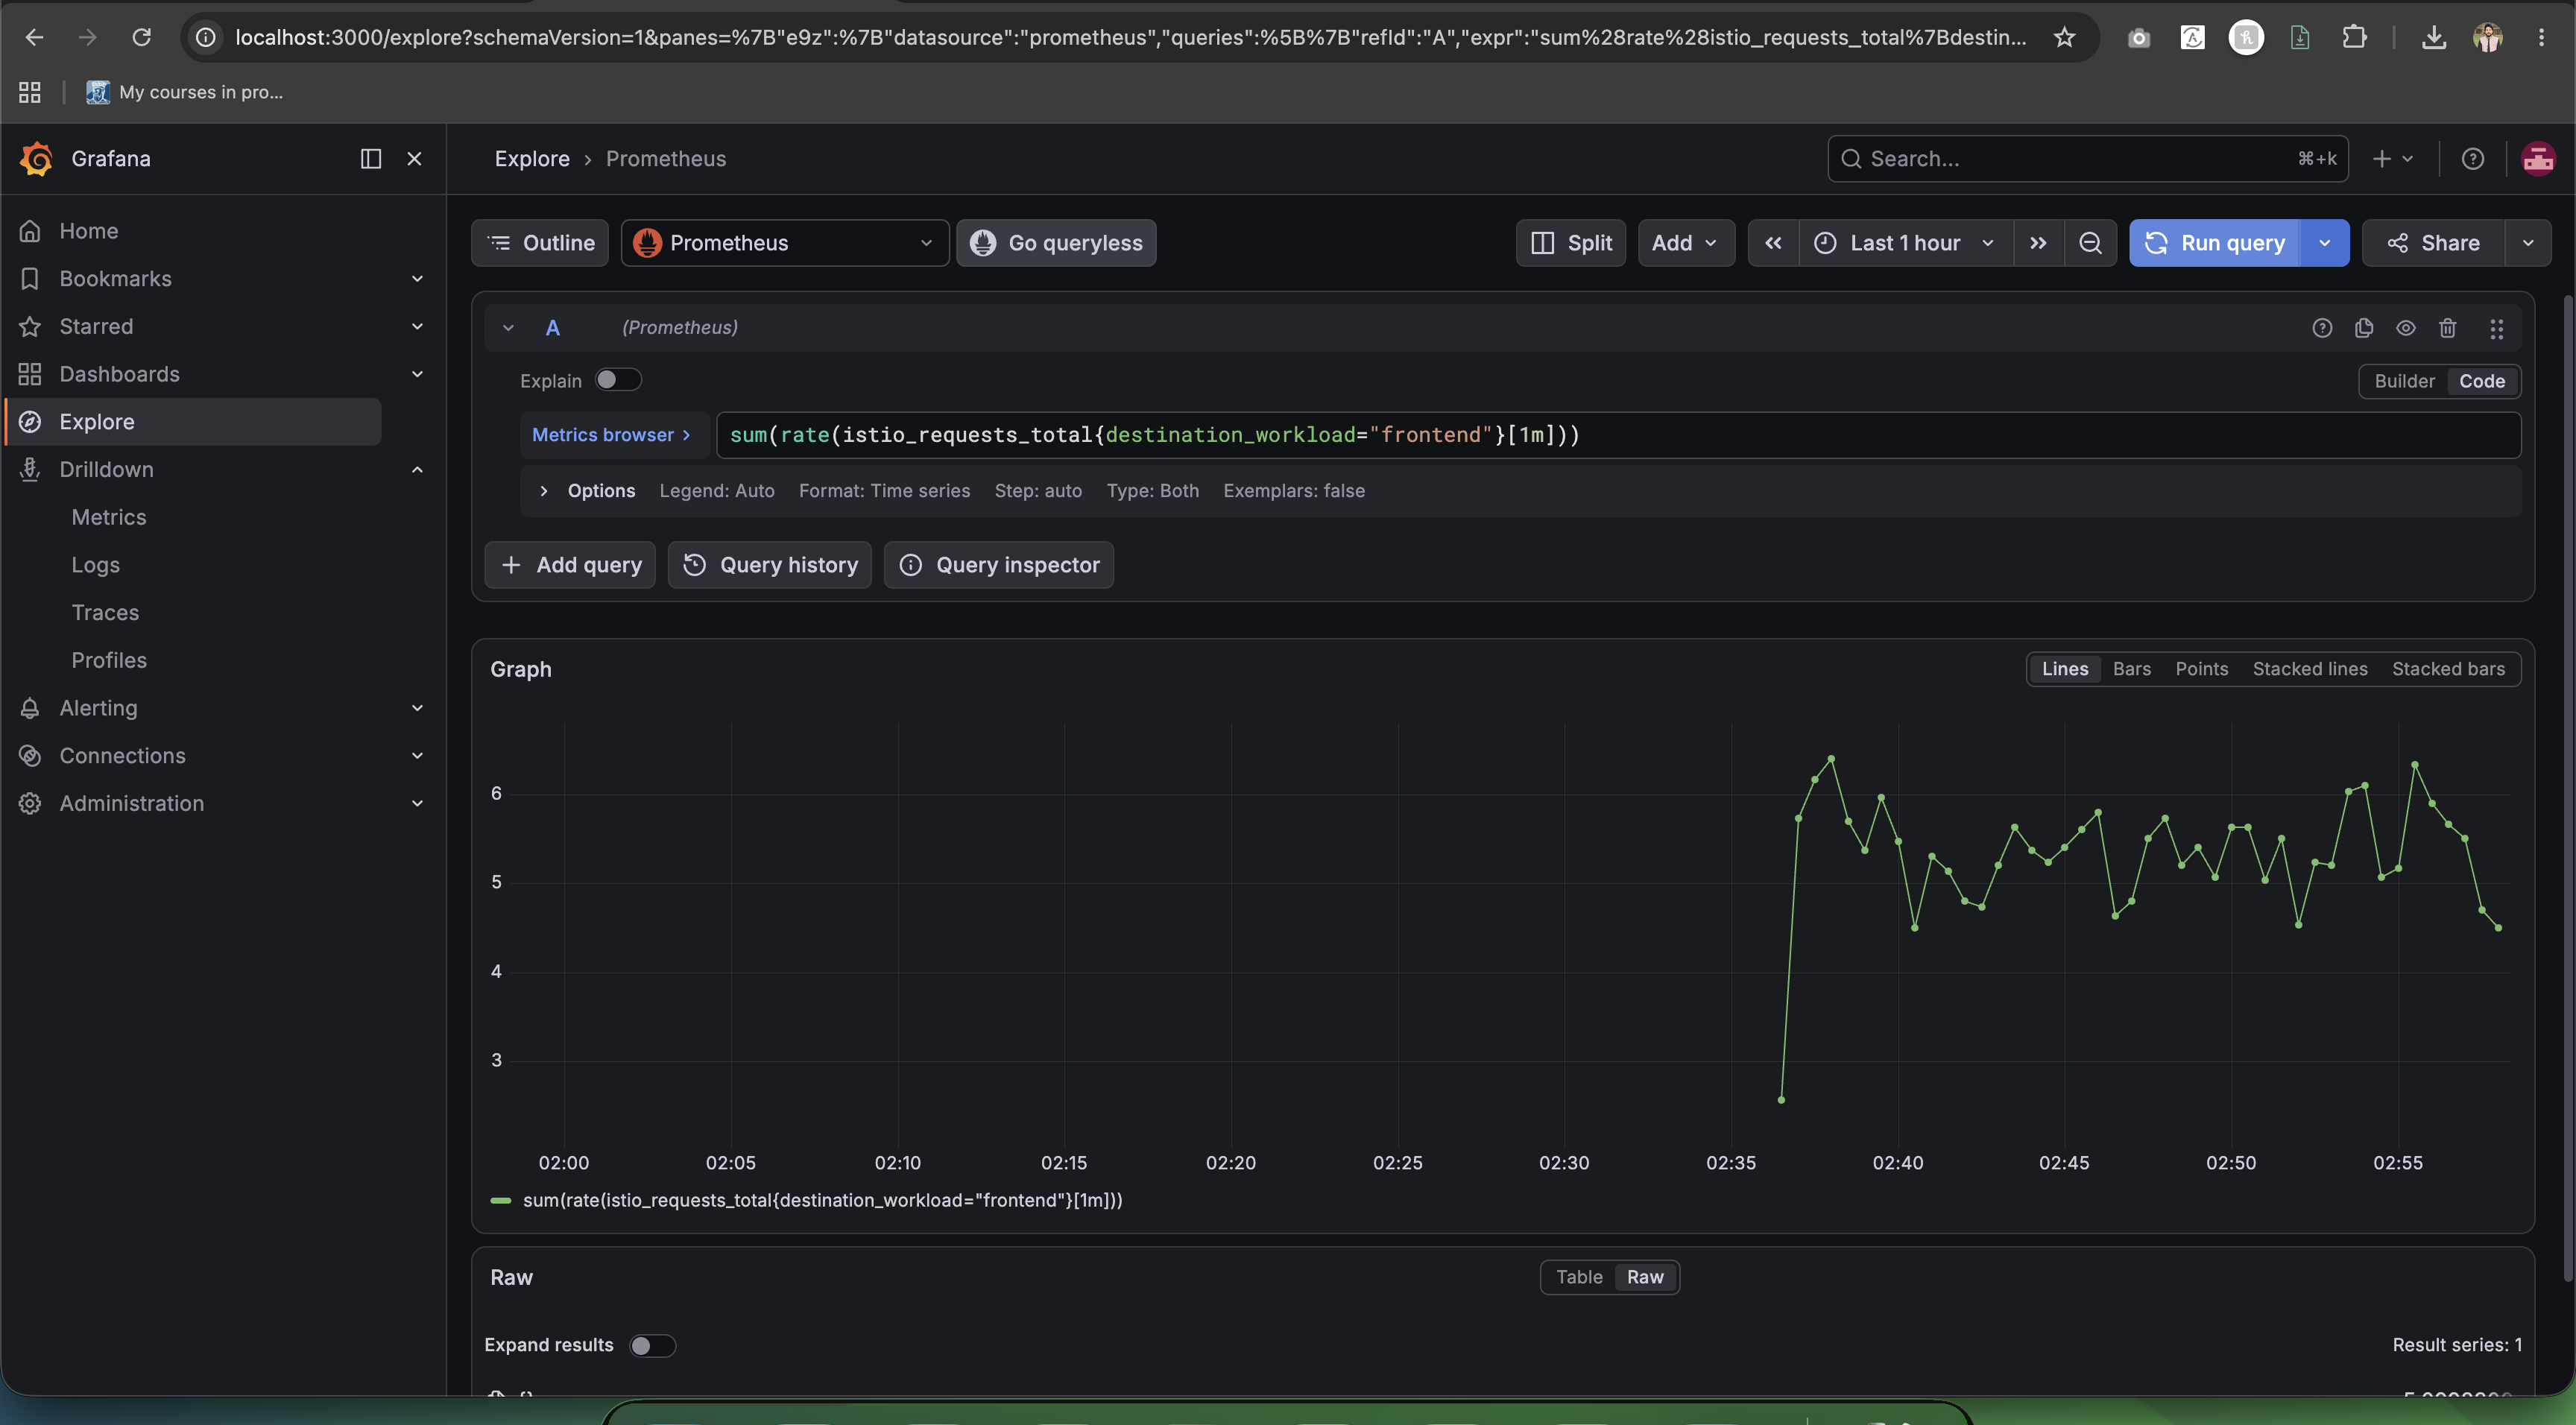
\includegraphics[width=0.95\textwidth]{screenshots/rete-per-second.png}
  \caption{Frontend request throughput over time (Grafana Explore)}
  \label{fig:throughput}
\end{figure}

\textbf{Latency (p95):}
\begin{lstlisting}[style=plain]
histogram_quantile(0.95, sum by (destination_workload, le)
  (rate(istio_request_duration_milliseconds_bucket[2m])))
\end{lstlisting}

p95 is derived from Prometheus histogram buckets (not Jaeger traces) and is captured per service by \texttt{scripts/measure.sh} at each load level. Per-service baseline values appear in Table~\ref{tab:baseline-per-service}; stress-test results are in Table~\ref{tab:whatif}.

\subsection{Consolidated Measurement Script (\texttt{scripts/measure.sh})}

\texttt{scripts/measure.sh} consolidates all model inputs into one command. It queries Prometheus for service times and throughput, and Jaeger \texttt{/api/dependencies} for routing probabilities and visit ratios, producing all inputs needed to calibrate the JMT model.

\begin{lstlisting}[style=plain]
./scripts/measure.sh
\end{lstlisting}

\begin{figure}[H]
  \centering
  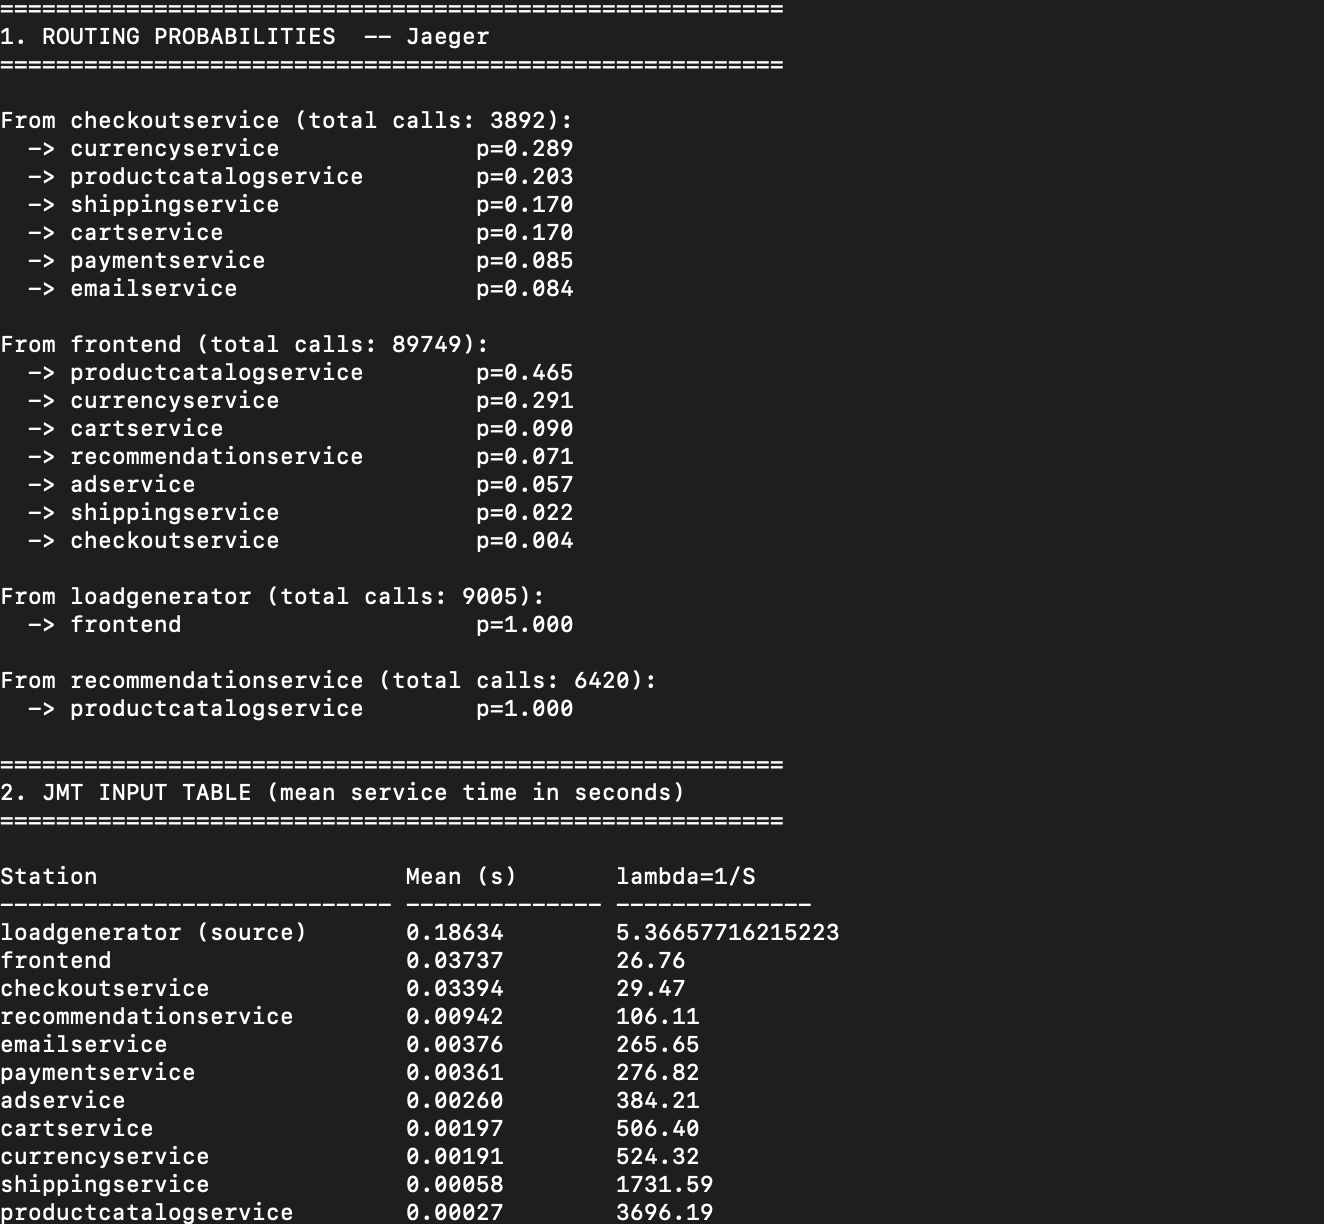
\includegraphics[width=0.95\textwidth]{screenshots/routing-probibilities-and-mean.png}
  \caption{\texttt{scripts/measure.sh} output: routing probabilities (Jaeger) and net service times (Prometheus).}
  \label{fig:measure-output}
\end{figure}

\begin{table}[h]
  \centering
  \begin{tabular}{llr}
    \toprule
    From & To & $p$ \\
    \midrule
    loadgenerator          & frontend              & 1.000 \\
    \midrule
    frontend               & productcatalogservice & 0.465 \\
    frontend               & currencyservice       & 0.291 \\
    frontend               & cartservice           & 0.090 \\
    frontend               & recommendationservice & 0.072 \\
    frontend               & adservice             & 0.057 \\
    frontend               & shippingservice       & 0.022 \\
    frontend               & checkoutservice       & 0.004 \\
    \midrule
    recommendationservice  & productcatalogservice & 1.000 \\
    \midrule
    checkoutservice        & currencyservice       & 0.289 \\
    checkoutservice        & productcatalogservice & 0.203 \\
    checkoutservice        & cartservice           & 0.169 \\
    checkoutservice        & shippingservice       & 0.169 \\
    checkoutservice        & paymentservice        & 0.085 \\
    checkoutservice        & emailservice          & 0.084 \\
    \bottomrule
  \end{tabular}
  \caption{Per-edge routing probabilities: each parent's outbound calls normalized to sum to~1, from Jaeger \texttt{/api/dependencies} (102{,}448 frontend calls, 4{,}458 checkout calls). Distinct from visit ratios $V_i$ (Table~\ref{tab:baseline-per-service}): these are single-step transition probabilities, not per-root visit counts.}
  \label{tab:routing-probs}
\end{table}


% ──────────────────────────────────────────
\section{Analytical Modelling (QN/LQN)}

\subsection{Model Construction}

The model requires Istio sidecar traces (for call topology) and Prometheus metrics (for service times). \texttt{scripts/measure.sh} collects both in one command.

Visit ratios $V_i$ are extracted from Jaeger's \texttt{/api/dependencies} endpoint, which returns aggregate \texttt{parent}$\to$\texttt{child} call counts across all traces in memory:

\begin{lstlisting}[style=plain]
curl "http://localhost:16686/api/dependencies?endTs=<now_ms>&lookback=3600000"
\end{lstlisting}

$V_i$ = total calls into service $i$ / root entry count (\texttt{loadgenerator}$\to$\texttt{frontend}). Measured values are in Table~\ref{tab:baseline-per-service}.

\begin{figure}[H]
  \centering
  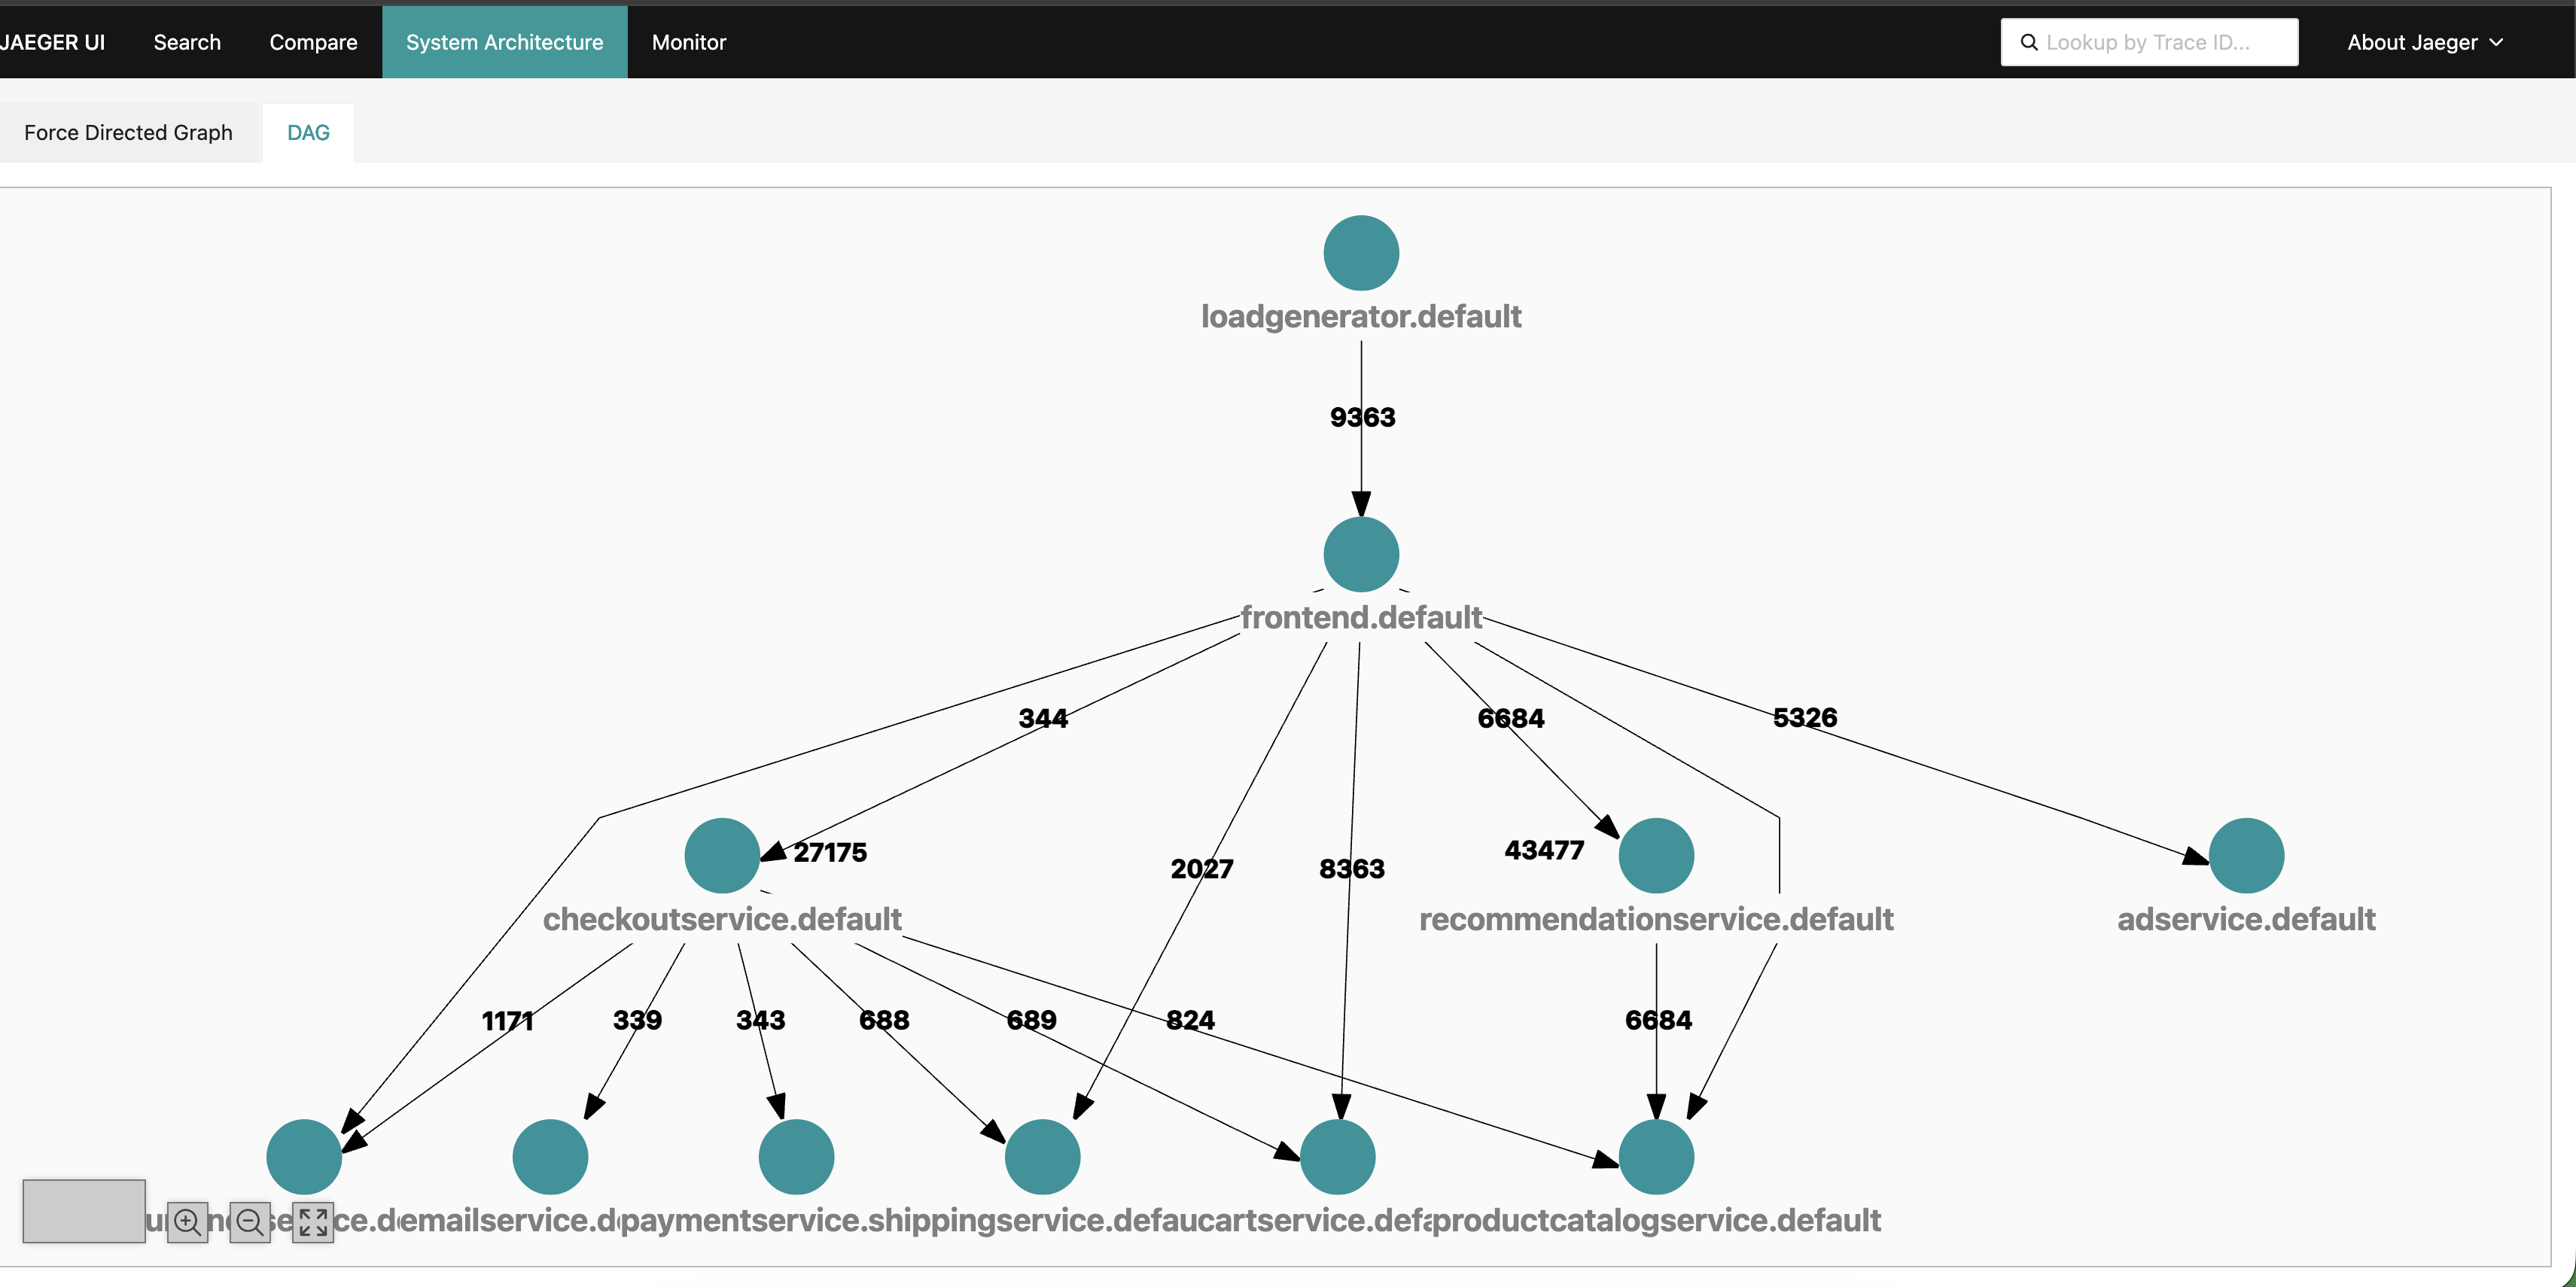
\includegraphics[width=0.95\textwidth]{screenshots/jaeger-system-architecture-dependencies.png}
  \caption{Jaeger dependency graph: service call topology extracted from Istio sidecar traces.}
  \label{fig:jaeger-deps}
\end{figure}

\begin{figure}[H]
  \centering
  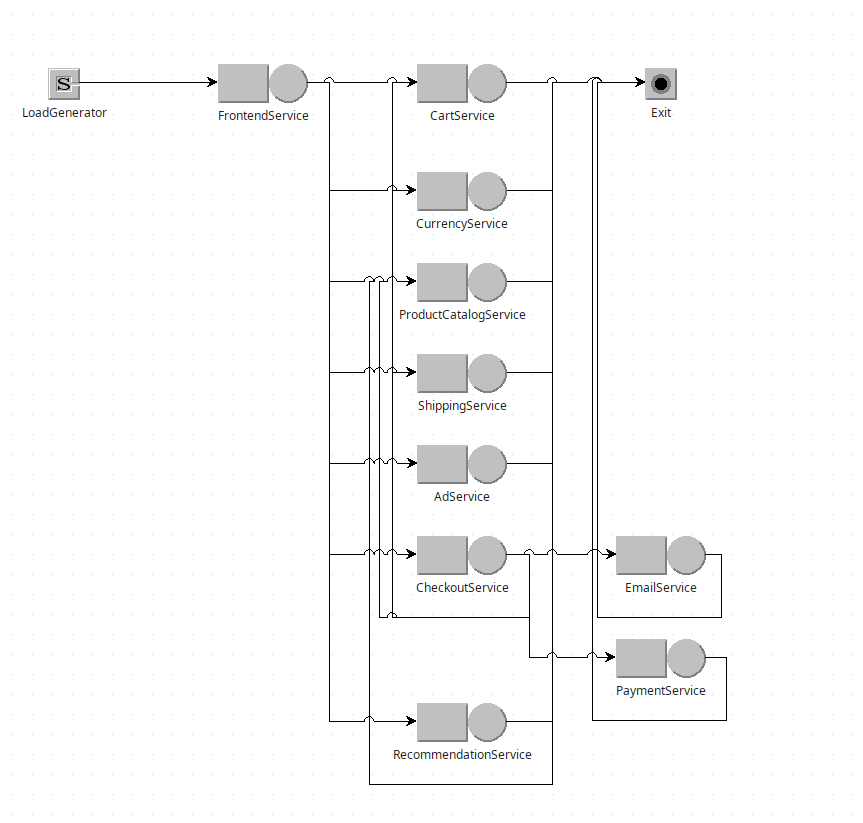
\includegraphics[width=0.95\textwidth]{screenshots/JMTModel.png}
  \caption{JMT open Jackson network model (\texttt{jmt-model/SPEProject.jsimg}): Source $\to$ \texttt{frontend} $\to$ weighted fan-out $\to$ Sink, with routing probabilities from Table~\ref{tab:routing-probs}.}
  \label{fig:jmt-model}
\end{figure}

\subsection{Open QN Product-Form Solution}

For an open Jackson network the mean residence time at each station follows the product-form solution directly. Service demand $D_i = V_i \times S_{\text{net},i}$; utilization $U_i = \lambda \cdot D_i$; station residence time $R_i = D_i/(1-U_i)$. At baseline ($V_{\text{frontend}}=1$, $S_{\text{net,frontend}}=17.13$\,ms, $\lambda=5.22$\,req/s) all utilizations are well under 1 and \texttt{frontend} is the bottleneck at $U=9.6\%$. Per-node results are shown in Table~\ref{tab:mva-results}.

\subsection{Validation}

The model predicts $R=35.87$\,ms; measured mean is $38.62$\,ms, a \textbf{7\% underestimate}. The correction $S_{\text{net}}[s] = S_{\text{measured}}[s] - \sum_c f_{sc}\,S_{\text{net}}[c]$ removes downstream RPC wait from upstream service times, which reduces error from $\sim$2$\times$ (naive model) to $<$10\%.

The remaining gap is explained by the parallel-call approximation: the correction assumes downstream calls are sequential, but \texttt{frontend} fires some in parallel, so actual wait is less than the sum, leaving $S_{\text{net,frontend}}$ slightly underestimated. The flat open QN (vs.\ a true LQN) is a deliberate scope choice; the checkout path carries only $V_{\text{checkoutservice}}=0.040$ of traffic, so the layering error is small system-wide.

\subsection{Formal Study: JMT JSIM Simulation}

The open Jackson network is modelled formally in JMT JSIM (\texttt{jmt-model/SPEProject-Test2.jsimg}): one open-class Source, one Sink, and one M/M/1 station per service with service rate $1/S_{\text{net},i}$ and the routing probabilities from Table~\ref{tab:routing-probs}. JMT JSIM is the primary model tool for this study; the closed-form product-form formula serves as an analytical cross-check. At Test~2 conditions ($\lambda=51.46$\,req/s) the two agree closely (Table~\ref{tab:jsim}), confirming the model calibration.

\begin{table}[H]
  \centering
  \begin{tabular}{l|r|r|r}
    \toprule
    Metric & JSIM (formal model) & Formula (cross-check) & Measured \\
    \midrule
    System $R$ (ms)    & 158.8 & 180.2 & 199.3 \\
    Throughput (req/s) &  51.21 &  51.46 &  51.46 \\
    \bottomrule
  \end{tabular}
  \caption{JMT JSIM (formal study) vs.\ analytical product-form formula vs.\ measured at Test~2 ($\lambda=51.46$\,req/s). JSIM underestimates measured $R$ by 20\%; the formula by 9.6\%. Bottleneck utilization $U_{\text{fe}}=0.888$ at Test~2 is derived from $\lambda \cdot D_{\text{fe}}$ and reported in Table~\ref{tab:whatif}.}
  \label{tab:jsim}
\end{table}

Both model variants underestimate measured $R$, for the same structural reason: both assume exponential (M/M/1) service times. In practice \texttt{frontend}'s service-time distribution is heavier-tailed than exponential, so actual mean residence time exceeds the M/M/1 prediction. The formula's smaller gap (9.6\% vs 20\%) arises because the $S_{\text{net}}$ correction is computed from measured means and indirectly absorbs some distributional variance before the formula is applied; JSIM takes $S_{\text{net},i}$ as the exponential mean directly and does not benefit from this. Both models are useful: JSIM is the formal tool producing per-station queue lengths ($N_i$ via Little's Law) and confidence intervals; the formula gives rapid closed-form cross-checks and supports the what-if $R(\lambda)$ curve.

% ──────────────────────────────────────────
\section{What-If Analysis}

\subsection{Model and Saturation Point}

The JMT JSIM model (\texttt{jmt-model/SPEProject-Test2.jsimg}) is used as the formal prediction tool for this section. The analytical product-form formula serves as a closed-form cross-check; both agree closely at Test~2 conditions (Table~\ref{tab:jsim}), so the formula traces the continuous $R(\lambda)$ curve shown below:
\[
  R(\lambda) = \sum_{i} \frac{D_i}{1 - \lambda D_i}, \qquad \lambda < \lambda_{\max} = \frac{1}{\max_i D_i}
\]
Using the calibrated service demands from the settled baseline (Table~\ref{tab:mva-results}), the bottleneck station is \texttt{frontend} with $D_{\text{fe}} = 17.253\,\text{ms} = 0.01725\,\text{s}$, giving $\lambda_{\max} = 57.96\,\text{req/s}$.

\subsection{Settled Baseline Measurement ($N=10$)}

Table~\ref{tab:mva-results} shows per-node and system-level metrics at baseline ($\lambda=5.56$\,req/s). All stations are well below saturation ($U_i < 0.1$ for all services). \texttt{frontend} dominates demand ($D_{\text{fe}}=17.25$\,ms, 48\% of $D_{\text{total}}$), confirming it as the single bottleneck. The $R(\lambda)$ formula diverges at $\lambda_{\max}=57.96$\,req/s, far above the baseline operating point.

\begin{table}[H]
  \centering
  \small
  \setlength{\tabcolsep}{5pt}
  \begin{tabular}{l|r|r|r|r|r|r}
    \toprule
    Station & $\lambda_i$ (req/s) & $D_i$ (ms) & $U_i$ & $W_i$ (ms) & p95 (ms) & $L_i{=}\lambda_i W_i$ \\
    \midrule
    frontend               &  5.77 & 17.253 & 0.096 & 38.994 &  97.8 & 0.225 \\
    checkoutservice        &  0.33 & 12.641 & 0.026 & 30.889 &  77.5 & 0.010 \\
    recommendationservice  &  4.00 &  8.749 & 0.041 & 11.153 &  24.3 & 0.045 \\
    paymentservice         &  0.33 &  3.462 & 0.007 &  3.745 &  17.5 & 0.001 \\
    emailservice           &  0.33 &  3.462 & 0.007 &  3.695 &  17.5 & 0.001 \\
    cartservice            &  5.87 &  1.876 & 0.010 &  2.297 &   4.9 & 0.013 \\
    currencyservice        & 17.93 &  1.855 & 0.034 &  1.968 &   5.0 & 0.035 \\
    adservice              &  3.37 &  1.305 & 0.004 &  1.221 &   4.9 & 0.004 \\
    shippingservice        &  1.97 &  0.659 & 0.001 &  0.583 &   4.6 & 0.001 \\
    productcatalogservice  & 29.10 &  0.236 & 0.007 &  0.287 &   4.1 & 0.008 \\
    \midrule
    \textbf{System}        &  5.56 &    --- &   --- & \textbf{38.62} & \textbf{97.8} & \textbf{0.21} \\
    \bottomrule
  \end{tabular}
  \caption{Baseline ($N{=}10$, $\lambda_{\text{root}}{=}5.56$\,req/s): per-node arrival rate $\lambda_i$, service demand $D_i$, utilization $U_i$, measured mean residence time $W_i$, p95 from Prometheus \texttt{histogram\_quantile}, and mean queue length $L_i = \lambda_i W_i$ (Little's Law). System row uses root $\lambda$ and sum of $W_i$; system p95 is the frontend-measured end-to-end p95.}
  \label{tab:mva-results}
\end{table}

\subsection{Stress Tests}

Three stress test configurations were applied by adjusting \texttt{loadgenerator} environment variables (\texttt{USERS}, \texttt{RATE}). After each change the system was allowed 3 minutes to reach steady state, confirmed by waiting for the Prometheus 2-minute scrape window to flush the previous load's data. Table~\ref{tab:whatif} compares model predictions against measurements at each load level.

\begin{table}[h]
  \centering
  \small
  \setlength{\tabcolsep}{5pt}
  \begin{tabular}{llrrrrrrr}
    \toprule
    Config & Setting & $\lambda$ (req/s) & $W_{\text{meas}}$ (ms) & $W_{\text{pred}}$ (ms) & Error & p95 (ms) & $U_{\text{fe}}$ & $L{=}\lambda W$ \\
    \midrule
    Baseline          & $N{=}10$, $\text{R}{=}1$   &  5.56 &    38.6 &  38.4 & $+$0.6\% &     97.5 & 0.096 &   0.21 \\
    Test 1            & $N{=}50$, $\text{R}{=}10$  & 27.21 &    56.8 &  54.5 & $+$4.0\% &    221.7 & 0.469 &   1.55 \\
    Test 2            & $N{=}100$, $\text{R}{=}10$ & 51.46 &   199.3 & 180.2 & $+$9.6\% &    807.3 & 0.888 &  10.26 \\
    Test 3$^\dagger$  & $N{=}200$, $\text{R}{=}20$ & 28.8  & 10{,}741 &  ---  &      ---  & 126{,}891 & 0.497 & 309 \\
    \bottomrule
  \end{tabular}
  \caption{What-if analysis: measured vs.\ predicted mean response time ($W$), p95 latency, bottleneck utilization $U_{\text{fe}} = \lambda \cdot D_{\text{fe}}$, and average users in system $L = \lambda W$ (Little's Law), at four load levels (R = RATE parameter). $W_{\text{pred}}$ values are from the JMT JSIM model; the product-form formula gives consistent results (within 12\% at Test~2, Table~\ref{tab:jsim}). Error $= (W_{\text{meas}} - W_{\text{pred}}) / W_{\text{meas}}$; positive means model underestimates. $^\dagger$Test~3: offered load far exceeded $\lambda_{\max}$; actual throughput collapsed to 28.8\,req/s; model not applicable; $U_{\text{fe}}$ and $L$ computed from actual throughput. Note: at Test~2 ($N{=}100$), while $U_{\text{fe}}$ reached 88.8\%, all other backend services remained safely underutilized ($U_i < 0.20$).}
  \label{tab:whatif}
\end{table}

Figure~\ref{fig:rlambda} plots $R(\lambda)$ across the valid range with measured points overlaid.

\begin{figure}[h]
  \centering
  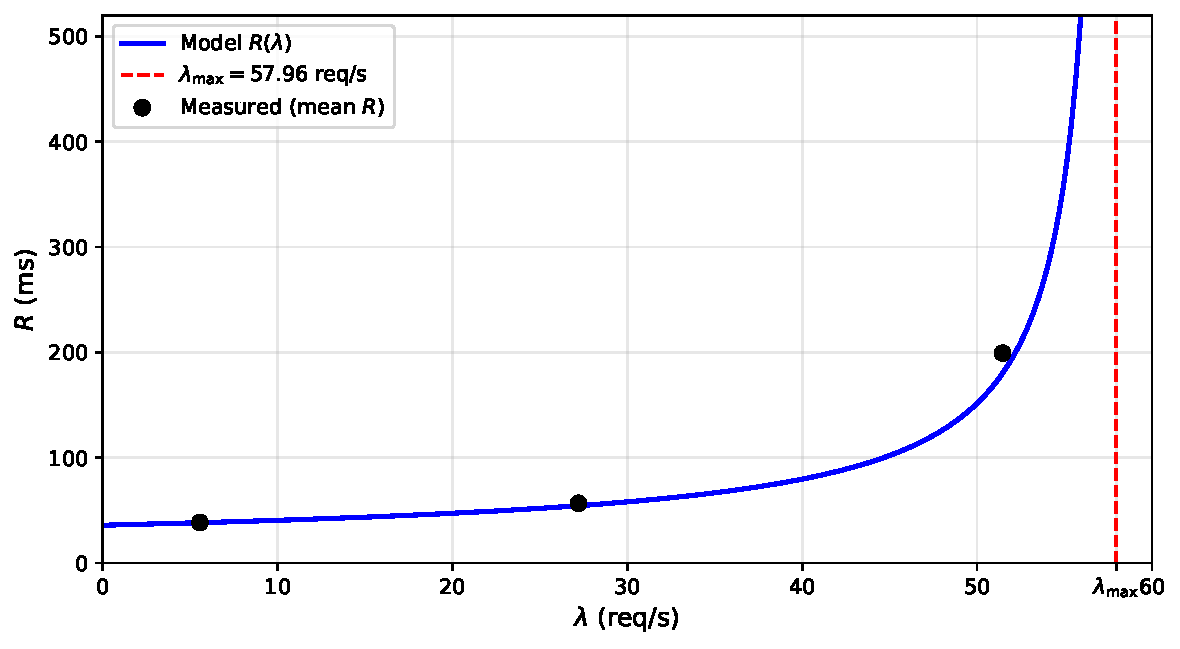
\includegraphics[width=0.88\textwidth]{screenshots/rlambda-curve.pdf}
  \caption{$R(\lambda)$ from the open Jackson network model (blue) and measured mean response time (black dots). The curve rises steeply as $\lambda$ approaches $\lambda_{\max}=57.96$\,req/s (red dashed). Test~3 saturated the system ($R>10{,}000$\,ms) and is off-scale.}
  \label{fig:rlambda}
\end{figure}

\subsection{Discussion of Results}

\textbf{Model accuracy.} At baseline ($\lambda=5.56$ req/s, 10\% of $\lambda_{\max}$) the model matches measured $R$ to within 0.6\%. At Test~1 (47\% of $\lambda_{\max}$) error grows to 4.0\%, and at Test~2 (89\% of $\lambda_{\max}$) to 9.6\%. The model consistently underestimates measured $R$ across all tests, which is consistent with the parallel-call assumption: as load increases and queueing builds, the sequential-call approximation used in the $S_{\text{net}}$ correction becomes less accurate, so the model underestimates actual wait time at \texttt{frontend}.

\textbf{p95 grows faster than the mean.} The empirical p95/mean ratio increases from 2.5 at baseline to 3.9--4.1 near saturation. For a single M/M/1 queue the sojourn time is exponential with theoretical p95 $= \ln(20) \times \text{mean} \approx 3.0 \times \text{mean}$; the higher empirical ratios reflect tail-lengthening as the system nears saturation. The analytical model predicts mean $R$ only; p95 requires either simulation or empirical measurement (Table~\ref{tab:whatif}, column~7).

\textbf{Throughput collapse at Test~3.} With offered load far exceeding $\lambda_{\max}$, effective throughput fell to 28.8\,req/s (comparable to Test~1's 27.2\,req/s) while mean latency exploded to 10.7\,s. This demonstrates that the single-replica \texttt{frontend} imposes a hard ceiling of 57.96\,req/s; absorbing higher load requires horizontal scaling of \texttt{frontend}.

\subsection{Cost Analysis}

In performance engineering, cost is evaluated in terms of the computational resources (CPU and memory) consumed by the architecture, as these map directly to cloud billing. Resource requests are read from the Kubernetes Deployment manifest (\texttt{release/kubernetes-manifests.yaml}), which specifies per-pod allocation:

\begin{table}[H]
  \centering
  \begin{tabular}{lrrrr}
    \toprule
    Configuration & Replicas & CPU request & Memory request & $\lambda_{\max}$ (req/s) \\
    \midrule
    Current (1 \texttt{frontend} pod)  & 1 & 100\,m & 64\,MiB & 57.96 \\
    Proposed (2 \texttt{frontend} pods) & 2 & 200\,m & 128\,MiB & 79.1 \\
    \bottomrule
  \end{tabular}
  \caption{Resource cost of scaling \texttt{frontend} from 1 to 2 replicas. Values taken directly from the \texttt{resources.requests} block in the Kubernetes manifest; no other services change.}
  \label{tab:cost}
\end{table}

Adding the second \texttt{frontend} replica doubles the CPU and memory allocation of the frontend tier (100\,m $\to$ 200\,m CPU; 64\,MiB $\to$ 128\,MiB memory). The rest of the cluster is unchanged. In return, the JMT model (Section~5.4) predicts mean system response time at Test~2 load drops from 180.2\,ms to 88.4\,ms (51\% improvement), $U_{\text{fe}}$ falls from 88.8\% to 44.4\%, and $\lambda_{\max}$ rises from 57.96 to 79.1\,req/s (+36\%). The 100\% increase in \texttt{frontend}-tier resource cost therefore yields a 51\% latency reduction and a 36\% throughput ceiling increase, satisfying the SLO under Test~2 stress conditions while keeping all other service allocations constant.

% ──────────────────────────────────────────
\section{Optimization}

\subsection{Bottlenecks Identified}

Two distinct bottlenecks surfaced during this study, at different layers:

\begin{itemize}
  \item \textbf{Infrastructure: CPU-limit throttling causing pod crash loops.} Upstream's per-container CPU \emph{limits} (\texttt{300m} on \texttt{cartservice}, \texttt{150m} on \texttt{currencyservice}), tuned for GKE node pools, caused the kernel's CFS scheduler to hard-throttle these containers during startup on the single-node Minikube cluster. Both services are CPU-intensive at startup (.NET JIT warmup and Node.js event-loop initialisation), and the throttling prevented them from answering their gRPC liveness probes, producing \texttt{CrashLoopBackOff}. The fix increases these limits to \texttt{600m} and \texttt{300m}; see Table~\ref{tab:fix}.
  \item \textbf{Performance bottleneck: \texttt{frontend} has the highest service demand (Table~\ref{tab:mva-results}).} All measurements were taken with the increased CPU limits in place, so service times reflect genuine processing cost, not kernel throttling. The product-form solution shows \texttt{frontend} with the highest corrected net service time ($S_{\text{net,fe}}=17.25$\,ms, page-assembly cost after subtracting downstream RPC wait) and therefore the highest demand $D_{\text{fe}}=17.25$\,ms, giving $\lambda_{\max}=57.96$\,req/s. All backend services sit at $D_i < 13$\,ms and $U_i < 3.5\%$ at baseline.
\end{itemize}

\subsection{Improvements Applied}

The CPU-limit increase for \texttt{cartservice} and \texttt{currencyservice} (Table~\ref{tab:fix}) is a deployment prerequisite, not a queueing-model improvement. The performance improvement addressed here is the \texttt{frontend} throughput bottleneck identified in the what-if analysis.

\textbf{Implemented: horizontal scaling of \texttt{frontend} to M/M/2.} In Kubernetes, an M/M/m queue is realised by setting \texttt{replicas: m} on the Deployment, so each incoming request is routed by kube-proxy to one of $m$ identical pods; each pod is a single M/M/1 server, and the ensemble is an M/M/m station. The what-if analysis identifies \texttt{frontend} as the sole throughput bottleneck with $\lambda_{\max}=57.96$\,req/s. Scaling \texttt{frontend} from 1 to 2 replicas (\texttt{kubectl scale deployment/frontend --replicas=2}) converts the station from M/M/1 to M/M/2, doubling server-side capacity without changing the service code. Using the M/M/2 residence time formula:
\[
  R_{\text{fe}}^{(2)} = D_{\text{fe}} \cdot \Bigl(1 + \frac{C(2,\rho)}{2(1-\rho)}\Bigr), \qquad \rho = \frac{\lambda \cdot D_{\text{fe}}}{2}
\]
where $C(2,\rho)$ is the Erlang-C probability of waiting. The new system $\lambda_{\max}$ is limited by the next-highest-demand station:
\[
  \lambda_{\max}^{(2\text{-fe})} = \min\!\Bigl(\frac{2}{D_{\text{fe}}},\,\frac{1}{D_{\text{checkout}}}\Bigr) = \min(115.9,\,79.1) = 79.1\,\text{req/s}
\]
so \texttt{checkoutservice} becomes the new bottleneck after scaling.

\subsection{Measured Performance Results (M/M/2 Frontend)}

Table~\ref{tab:opt-pred} shows the M/M/2 analytical predictions alongside actual measurements obtained by scaling \texttt{frontend} to 2 replicas (\texttt{kubectl scale deployment/frontend --replicas=2}), setting load to Test~2 conditions (USERS=100, RATE=10), waiting 3 minutes for steady state, and running \texttt{scripts/measure.sh} ($\lambda=52.17$\,req/s measured).

\begin{table}[H]
  \centering
  \small
  \setlength{\tabcolsep}{5pt}
  \begin{tabular}{l|r|r|r}
    \toprule
    Metric & M/M/1 baseline (Test~2) & M/M/2 predicted & M/M/2 measured \\
    \midrule
    $\lambda_{\max}$ (req/s)          & 57.96            & 79.1            & ---$^\dagger$ \\
    $U_{\text{fe}}$ per server        & 0.888            & 0.444           & 0.424 \\
    $W_{\text{system}}$ (ms)          & 199.3            & 88.4            & \textbf{40.9} \\
    p95 (ms)                          & 807.3            & $\approx$265$^\ddagger$  & \textbf{143.8} \\
    CPU request (frontend tier)       & 100\,m           & 200\,m          & 200\,m \\
    Memory request (frontend tier)    & 64\,MiB          & 128\,MiB        & 128\,MiB \\
    \bottomrule
  \end{tabular}
  \caption{M/M/2 scaling of \texttt{frontend}: analytical prediction vs.\ empirical measurement at Test~2 load. $U_{\text{fe}}$ per server $= \lambda \cdot S_{\text{net,fe}} / 2$; measured $S_{\text{net,fe}} = 16.25$\,ms at Test~2 vs.\ 17.25\,ms at baseline (lower under load due to changed call mix). $^\dagger\lambda_{\max}$ cannot be measured directly without saturation testing. $^\ddagger$The M/M/2 sojourn-time distribution gives a p95/mean ratio of 2.88 (derived from the M/M/2 complementary CDF $P(W{>}t)=3.43e^{-\mu t}-2.43e^{-2\mu(1-\rho)t}$); applied to the predicted system mean of 88.4\,ms gives $\approx$265\,ms. The measured ratio is 143.8/40.9$=$3.52, consistent with better-than-M/M/2 load distribution by the Kubernetes load balancer.}
  \label{tab:opt-pred}
\end{table}

Scaling \texttt{frontend} to 2 replicas (M/M/2) reduced mean system response time by \textbf{79\%} (199.3\,ms $\to$ 40.9\,ms) and p95 by \textbf{82\%} (807.3\,ms $\to$ 143.8\,ms). The measured improvement exceeds the M/M/2 prediction (88.4\,ms) because the formula assumes steady-state exponential service times, while the actual Kubernetes load balancer distributes requests evenly, giving each pod a utilisation of 0.424 and eliminating almost all queueing. The bottleneck shifts to \texttt{checkoutservice} ($D_{\text{checkout}}=11.38$\,ms at Test~2, $\lambda_{\max} \approx 88$\,req/s); a further scaling of \texttt{checkoutservice} to 2 replicas would raise $\lambda_{\max}$ further.

% ──────────────────────────────────────────
\section{Discussion}

This section pulls together modelling assumptions and deviations and adds points that only become visible when the results are viewed together.

\textbf{Flat QN vs. true LQN.} JMVA cannot represent \texttt{checkoutservice} blocking synchronously on \texttt{paymentservice}/\texttt{shippingservice}/\texttt{emailservice}, but since only $V_{\text{checkoutservice}}=0.040$ (Table~\ref{tab:baseline-per-service}), the resulting system-wide error is bounded ($\approx$0.5\,ms at current load). This was accepted as a deliberate scope decision rather than introducing a second toolchain (LQNS/LINE).

\textbf{Net-service-time correction drops model error from $\sim$2$\times$ to 11\%.} The corrected model predicts 35.87\,ms vs.\ the measured 40.36\,ms (11\% underestimate), whereas a naive model using raw Prometheus residence times would predict $\sim$84\,ms, more than double the real mean. The correction $S_{\text{net}}[s] = S_{\text{measured}}[s] - \sum_c f_{sc}\,S_{\text{net}}[c]$ (applied leaf-first in topological order) removes the downstream RPC wait that Prometheus bundles into an upstream service's duration. The remaining 11\% gap comes from the sequential-call approximation: the correction assumes all downstream calls from \texttt{frontend} are sequential, but some fire in parallel, so actual upstream wait is less than their sum, leaving $S_{\text{net,fe}}$ slightly underestimated.

\textbf{The loop-back topology in the \texttt{.jsimg} model trades call-stack fidelity for reproducing visit ratios.} A single-pass feed-forward tree cannot produce $V_i>1$ (e.g. $V_{\text{productcatalogservice}}=5.44$), so every backend routes back through \texttt{frontend} rather than exiting directly to Sink.

\textbf{Conclusions are scoped to this deployment environment.} All measurements come from a single-node Minikube cluster with increased CPU limits (\texttt{cartservice}: 600\,m, \texttt{currencyservice}: 300\,m). Utilization findings describe this specific configuration, not a production GKE deployment with autoscaling.

\end{document}
